\documentclass{article}
\usepackage{fontspec}
% \setmainfont{Open Sans}
% \setmainfont{Times New Roman}

% TODO: Make sure Greek characters are showing

% TODO: Marissa question: My aloe plant is blooming! And reproducing! I haven't really figured out how they work yet... in particular, it seems perfectly capable of asexual reproduction as evidenced by the three pups appearing in the soil... so what are the flowers for?

\usepackage[hidelinks]{hyperref}

\usepackage{amsmath}
\usepackage{fullpage}
\usepackage{inconsolata}
\usepackage{graphicx}
\usepackage{minted}
\usepackage[sort&compress,numbers]{natbib}
\usepackage{optidef}
\usepackage{parskip}
\usepackage{pgfplots}
\usepackage{verbatim}

\setmonofont{Noto Sans Mono}

\pgfplotsset{compat=1.17}
\usetikzlibrary{patterns}

\renewcommand{\sectionautorefname}{\textsection}
\renewcommand{\subsectionautorefname}{\textsection}
\renewcommand{\subsubsectionautorefname}{\textsection}
% \renewcommand*{\thesection}{\textsection}
% \let\subsectionautorefname\sectionautorefname
% \let\subsubsectionautorefname\sectionautorefname

\hypersetup{pdfauthor={Richard Barnes (ORCID: 0000-0002-0204-6040)},%
            pdftitle={Finding Optimal Life Histories With Mathematical Programming},%
%            pdfsubject={Whatever},%
            pdfkeywords={TODO},%
            pdfproducer={LaTeX},%
            pdfcreator={pdfLaTeX}
}

\title{Finding Optimal Life Histories With Mathematical Programming}
\author{Richard Barnes}
\date{}

\begin{document}

\maketitle

\tableofcontents

\section{Introduction}

An organism's life history is the sequence of events related to survival and reproduction that occur from birth through death. Considered another way, an organism's life history is the time series of how it allocates energy and resources over its lifespan. We expect that allocation strategies of an organism are shaped by evolution to maximize reproductive fitness.

%TODO: Move away from policy function language
%TODO: X is everything the organism knows and is
%TODO: "current allocations and antitipcated needs" might need to be grouped better
In modeling life history, we would like to recover a policy function $\pi(X,t)$ which, given the organism's current allocations and anticipated future needs $X$, determines how incoming energy at time $t$ should be allocated. Finding such a function is challenging and the field has typically relied on optimal control theory and applications of Pontryagin's maximum principle to do so. This has required increasing mathematical sophistication over time~\citep{mirmirani_competition_1978, iwasa_optimal_1989, pugliese_optimal_1990, mironchenko_optimal_2014}. This paper recasts previous theory in the form of convex optimization problems which can be solved numerically. This has several advantages:
\begin{itemize}
\item Lower barriers to entry. Applying optimal control theory requires significant mathematical sophistication. This barrier to entry makes it unnecessarily challenging for ecologists to include theory in their work.
\item Faster ideation and exploration. Even for those who have mastered the techniques of optimal control theory, applying it to a particular case can still be time-consuming and seemingly simple modifications to a model can rapidly move it into the realm of intractibility. The techniques here make it easy to investigate model variants quickly.
\item Powerful solvers. The techniques presented here rely on a powerful toolbox of solvers which can quickly find optimal numerical solutions to even large problems. This means that instantiating seemingly complex problems in computer code is easy, even for beginners.
\item Guarantees. Most of the examples in this paper translate life history problems defined by differential equations into convex optimization problems. The solvers for these problems have several desirable properties. (1)~If a problem is non-convex, the solver can detect this and refuses to attempt a solution. (2)~If the problem is convex the solver is guaranteed to either find the optimal solution or return a certificate that the problem is either unbounded (arbitrarily good solutions are possible) or infeasible (no solution is possible).
\end{itemize}

% The paper is laid out as follows.
% \begin{itemize}
% \item \autoref{sec:mathprog} lays out the framework of mathematical programming.
% \item \autoref{sec:problems} presents a menagerie of problems TODO
% \item TODO
% \end{itemize}


%TODO: Make sure capitalization is consistent
%TODO: Is it good to have acronyms in ToC, but (LP), (CP) in

\section{Mathematical Programming}
\label{sec:mathprog}

\begin{figure}
\centering

\includegraphics[width=3in]{imgs/hierarchy-of-convex-programs.png}
\caption{The hierarchy of convex programming showing Linear Programming (LP), Quadratic Programming (QP), Second-Order Cone Programming (SOCP), Semi-definite Programming (SDP), and Convex Programming (CP). \label{fig:hierarchy}}
\end{figure}

The basic idea behind \textit{mathematical programming} is that we will specify an \textit{objective function} whose value we wish to minimize (or maximize) by finding the best values of a set of \textit{decision variables} whose values are subject to \textit{constraints} which combine the decision variables and \textit{parameters} (fixed numeric values which may vary from one instance of the problem to the next) using standard mathematical functions and either inequalities ($<,\le,\ge,>$) or equalities ($=$). Once the objective and constraints have been specified, we can pass the problem off a powerful software program called a solver which determines the optimal values of the decision variables.

Unfortunately, except for special cases, solving mathematical programs is extremely hard. Fortunately, the special cases are vast and include many problems of interest. Below we discuss some special cases of interest here moving from the most- to least-constrained problem space, as shown in \autoref{fig:hierarchy}.

\subsection{Linear Programming}

The simplest case is \textit{linear programming}. In a linear program, the objective and every constraint consists of linear equations. \autoref{fig:graphical_linear} shows a graphical representation of a particular linear program described below and hints out how it might be solved.

Imagine we have a plant whose reproductive success is determined by the biomass of its roots and leaves. The plant's goal is to grow so that the amount of root and leaf biomass it has maxmizes its reproductive output. The particular amounts of biomass it produces are its strategy.

\begin{figure}
  \centering
  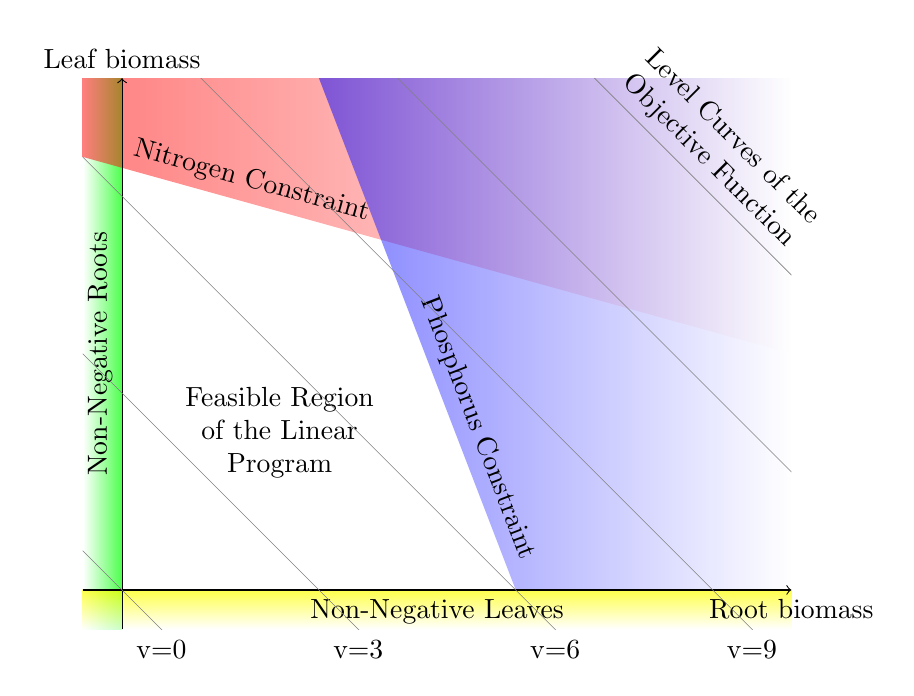
\begin{tikzpicture}
    \begin{scope}
      \shade[right color=green, left color=white, opacity=0.7] (-0.5,-0.5) rectangle (0,6.5);
      \node[rotate=90, above] at (0,3) {Non-Negative Roots};
      \shade[top color=yellow, bottom color=white, opacity=0.7] (-0.5,-0.5) rectangle (8.5,0);
      \node[below] at (4,0) {Non-Negative Leaves};
      \shade[left color=red, bottom color=red, right color=white, opacity=0.5] (-0.5,5.5) -- (8.5,3) -- (8.5,6.5) -- (-0.5,6.5) -- cycle;
      \path (-0.5,5.5) -- node[pos=0.23, sloped, above] {Nitrogen Constraint} (8.5,3);
      \shade[left color=blue, right color=white, opacity=0.5] (2.5,6.5) -- (8.5,6.5) -- (8.5,0) -- (5,0) -- cycle;
      \path (5,0) -- node[pos=0.3, sloped, above] {Phosphorus Constraint} (2.5,6.5);
      \node[text width=7em, align=center] at (2,2) {Feasible Region of the Linear Program};
      \draw[->] (-0.5,0) -- (8.5,0) node[below] {Root biomass};
      \draw[->] (0,-0.5) -- (0,6.5) node[above] {Leaf biomass};
      \node[rotate=-45, above, text width=9em, align=center] at (7.25,5.25) {Level Curves of the Objective Function};
      \node[above, text width=9em, align=center] at (0.5,-1) {v=0};
      \node[above, text width=9em, align=center] at (3,-1) {v=3};
      \node[above, text width=9em, align=center] at (5.5,-1) {v=6};
      \node[above, text width=9em, align=center] at (8,-1) {v=9};
      \path[clip] (-0.5,-0.5) rectangle (8.5,6.5);
      \foreach \i in {0.5,3,...,13} {
        \draw[help lines] (-0.5,\i) -- +(-45:15);
      }
    \end{scope}
  \end{tikzpicture}
  \caption{A graphical representation of a linear program.\label{fig:graphical_linear}}
  \end{figure}

If we were to plot aspects of this plant, we could do so by putting root biomass ($R$) on the x-axis and leaf biomass on the y-axis ($L$). With no further information, the space of possible solutions therefore spans the entire R-L plane. Obviously, though, no part of our plant cannot have negative biomass, so we add the constraints $R\ge0$ and $L\ge0$. This rules out three quadrants of the plane, which we indicate by adding green and yellow shading to \autoref{fig:graphical_linear}. The best strategy for our plant, whatever it is, must lie in the upper right quadrant. Now, let us say that a plant requires phosphorus $P$ to produce its leaves and roots and that the phosphorus requirements of the two differ; this implies the constraint $aR+bL\le P$. This constraint rules out any solution in the blue-shaded region. A similar constraint might apply to nitrogen, ruling out solutions in the red-shaded region.

Having come this far, we now have a clearly defined \textit{feasible region}, shown in white in \autoref{fig:graphical_linear}. The best strategy of the plant must lie somewhere in this region because any strategy outside of it would violate at least one constraint.

Finally, let us say that reproductive output, formally known as the objective function, is some linear function $cR+bL$ of leaf and root biomass---if this seems overly simplistic, remember, this is an example to illustrate mathematics, not a model we are actually interested in using. If we consider the level curves of the objective function---the lines obtained in \autoref{fig:graphical_linear} by taking $cR+bL=0$, $cR+bL=3$, and so on---we see that they define both a gradient and intersect the constraints.

With some reflection, we can see that the maximum value of the objective function must occur at the intersection of two or more constraints. It is obvious from the picture that the objective value cannot have a maximum value in the interior of the feasible region since it has a gradient there and any point in the interior is adjacent to another interior or boundary point that would be farther along this gradient. Therefore, we know the objective is maximized on the boundary. The isolines of the objective could be exactly parallel to one of the boundary segments, but, in this case, both end points of the segment will have the same objective value and we can choose on arbitrarily.

%https://upload.wikimedia.org/wikipedia/commons/d/d4/Simplex-method-3-dimensions.png
\begin{figure}
\centering
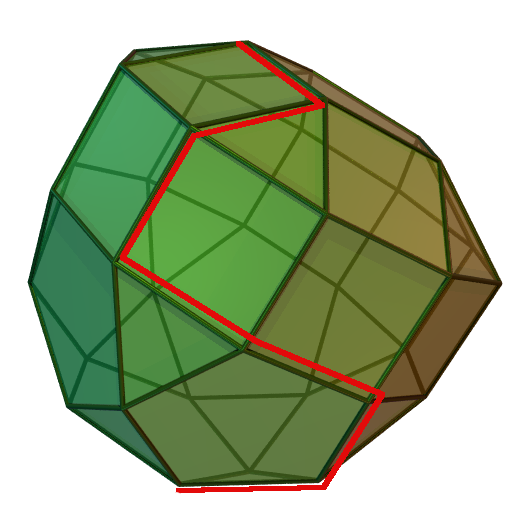
\includegraphics[width=3in]{imgs/Simplex-method-3-dimensions.png}
\caption{The simplex method in three dimensions.\label{fig:simplex}}
\end{figure}

This implies a simple algorithm for solving linear programs: find any vertex on the boundary, consider vertices linked to it by constraints, move to the vertex with the highest objective value, and repeat until no neighbouring vertex is better than the one you're at. As shown in \autoref{fig:simplex}, in higher dimensions the feasible region is bounded by planes or hyperlanes and the feasible region, rather than being a polygon, is called a polytope. Still, the algorithm is the same: find a vertex and walk along edges until the best vertex is found.

The algorithm described above is called the \textit{simplex algorithm}. Interestingly, while it is known that all linear programs can be solved efficiently (ie, in polynomial time) using another technique called the ellipsoidal algorithm, there are problems for which the simplex algorithm will perform very badly. In practice, however, these problems are rare and must be deliberately constructed. It's been said that at one point more compute power was devoted to running the simplex algorithm than any other program---a testament both to the practical value of the algorithm as well as linear programming itself.


\subsection{Convex Programming}
\label{sec:convex_programming}

\begin{figure}
\centering
\begin{tabular}{cc}

\includegraphics[height=1in]{imgs/potato.jpg} &

\includegraphics[height=1in]{imgs/banana.png}
\end{tabular}
\caption{Examples of a convex space (a potato) and a non-convex space (a banana).\label{fig:convexfoods}}
\end{figure}

As \autoref{fig:convexfoods} shows, the mathematical difference between a potato and a banana is that the potato is convex whereas the banana is non-convex; that is, any two points within the potato can be connected with a line which does not pass outside of the potato. In contrast, the banana contains points which can only be connected by a line passing outside of the banana.

Some reflection on our linear programming example reveals that the feasible region of a linear program is always a convex polytope. This is not an accident. If we draw isolines over a banana-shaped region, we find vertices of equal value that cannot be reached from each other. In such a situation the simplex algorithm no longer works and we have entered the \textit{much} harder-to-solve space of non-convex programming. While every convex problem is, in some sense, the same, each non-convex problem is non-convex in its own way. %TODO: Is this a good place for this?

Convexity is key to efficient mathematical programming. Since the intersection of two convex sets is itself a convex set, we can compose convex objects to form feasible spaces with properties that make them amenable to efficient maximization. Unfortunately, we don't know efficient solution algorithms for all convex objects, so in practice we often have to find a way to re-express our problems using convex forms that we know.

Classes for which we do have efficient algorithms in include:
\begin{itemize}
\item \textit{Linear programs (LP)}, as above.
\item \textit{Quadratic programs (QP)}, which includes linear programming as a special case, and is the class of all programs with linear constraints and an objective function of the form $\frac{1}{2}x^T Q x + q^T x$ where $Q$ is a constant matrix, $q$ is a constant vector, and $x$ is a vector variable.
\item \textit{Quadratically constrained quadratic programs (QCQP)}, which are similar to quadratic programs, but may include quadratic constraints.
\item \textit{Second-order cone programs (SOCP)}, which can have linear or quadratic objectives and constraints of the form $\lVert Ax+b\rVert_2 \le cx+d$, where $A$ is a constant matrix, $b$ and $c$ are constant vectors, $d$ is a constant, and $x$ is a variable vector.
\item \textit{Semi-definite programs (SDP)} where we wish to find a positive semi-definite matrix that satisfies an objective and constraints.
\item \textit{Relative Entropy Programming (EXP)}, a subset of cone programming (CP) containing SOCPs defined by constraints of the form $ye^{xy}\le z, y>0$. See \citet{Chandrasekaran2017} for an overview.
\item \textit{Power Cone Programming (POW)}, defined by constraints of the form $\prod_i x_i^{\alpha_i} \ge \sqrt{\sum_i x_i^2}, x_i\ge0$. %TODO: Find an overview Look at examples here: https://docs.mosek.com/modeling-cookbook/powo.html
\item \textit{Geometric Programming (GP)}, geometric programming is defined by an objective $f_0(x)$ and constraints $f_i(x)\le1$ and $g_j(x)=1$ where $f$ are posynomials and $g$ are monomials. Monomials take the form $c x_1^{a_1} x_2^{a_2}\ldots$ with $c>0$ and $a_i\in\mathcal{R}$. Posynomials are sums of monomials. A good review of geometric programming is given by \citet{Boyd2007}.
%\item \textit{Quasi-convex programming}, TODO
\end{itemize}

As detailed below, LPs are the easiest and fastest programs to solve and can include millions of variables and constraints. QP and QCQP programs are harder, so the programs we can solve with them are smaller. SOCP is harder still, but still very do-able using even free software, though the size of the programs we can solve is somewhat smaller. SDPs, EXP, and POW are active areas of research and even relatively small problems can be difficult.

The most exotic programs we'll use in this paper are SOCPs. %TODO: Check this

\subsection{Mixed-Integer Programming}

Integer programming (IP) arises when an optimization problem has one or more variables which are constrained to take only integer values. When such variables are mixed with continuous linear variables we have Mixed-Integer Linear Programming (MILP). If second-order cones are involved, then we have a MISOCP. The general class of such problems---those with both discrete and continuous variables---is called mixed-integer programming (MIP).

Integer programming belongs to a class of problems called NP for which there are no known efficient algorithms and for which many people think there will \textit{never} be efficient algorithms. Nonetheless, many solvers are able to solve small instances of integer problems, but often only at the cost of substantial compute time. In this paper we try to avoid MIPs when we can or limit the number of discrete variables when we can't. %TODO: Check this

\subsection{Solvers}

\begin{table}
\centering
\begin{tabular}{l|c|c|c|c|c|c|c|l}
Solver & LP  & QP  & SOCP & SDP & EXP & POW & MIP & Cost \\
CBC\footnote{\url{https://projects.coin-or.org/Cbc}}                                                                          & X   &     &      &     &     &     & X   & Free \\
GLPK\footnote{\url{https://www.gnu.org/software/glpk/}}                                                                       & X   &     &      &     &     &     &     & Free \\
GLPK\_MI\footnote{\url{https://www.gnu.org/software/glpk/}}                                                                   & X   &     &      &     &     &     & X   & Free \\
OSQP\footnote{\url{https://osqp.org/}}                                                                                        & X   & X   &      &     &     &     &     & Free \\
CPLEX\footnote{\url{https://www-01.ibm.com/software/commerce/optimization/cplex-optimizer/}}                                  & X   & X   & X    &     &     &     & X   & Free for Academics, \$199/mo \\
NAG\footnote{\url{https://www.nag.co.uk/nag-library-python/}}                                                                 & X   & X   & X    &     &     &     &     & \\
ECOS\footnote{\url{https://www.embotech.com/ECOS}}                                                                            & X   & X   & X    &     & X   &     &     & Free \\
GUROBI\footnote{\url{http://www.gurobi.com/}}                                                                                 & X   & X   & X    &     &     &     & X   & Free for Academics, \$\$ \\
MOSEK\footnote{\url{https://www.mosek.com/}}                                                                                  & X   & X   & X    & X   & X   & X   & X$^*$ & \$2,050 + \$512/yr\\
CVXOPT\footnote{\url{http://cvxopt.org/}}                                                                                     & X   & X   & X    & X   &     &     &     & Free \\
SCS\footnote{\url{http://github.com/cvxgrp/scs}}                                                                              & X   & X   & X    & X   & X   & X   &     & Free \\
SCIP\footnote{\url{https://scip.zib.de/}}                                                                                     & X   & X   & X    &     &     &     & X   & Free \\
XPRESS\footnote{\url{https://www.fico.com/en/products/fico-xpress-optimization}}                                              & X   & X   & X    &     &     &     & X   & Free for Academics, \$\$ \\
\end{tabular}
\caption{Solvers for mathematical programming and their capabilities. (*) Except mixed-integer SDP.\label{tbl:solvers}}
\end{table}
%(From [CVXPY documentation](https://www.cvxpy.org/tutorial/advanced/index.html#choosing-a-solver))


\autoref{tbl:solvers} lists various open source and commercial solvers. As discussed in \autoref{sec:convex_programming}, there is a gradient to the ease with which problems can be solved. Even large instances of linear programs can be solved for free by any of a large variety of software. In constrast, if we wish to solve an MISOCP problem, the only free options are SCIP, XPRESS, and CPLEX. Obtaining a CPLEX academic license is challenging and SCIP is brutally slow for this sort of problem, leaving XPRESS as the only viable option. In this paper, we focus on classes of problems for which good solvers are available.

\subsection{Domain Specific Languages}

Domain Specific Languages (DSLs) are programming languages or libraries that are designed to make expressing a particular type of problem easier. All of the solvers mentioned above have their own DSL, but using the solver's DSL directly means you're stuck with that solver even if it turns out not to work well for your particular problem. Fortunately, there are DSLs which allow you to express problems in such a way that they are easily passed to \textit{any} solver. In this paper we will use two DSLs both for practical purposes (sometimes one works better than the other) as well as to demonstrate the generic nature of the methods we discuss.
\begin{itemize}
\item \textbf{cvxpy} (\url{https://www.cvxpy.org/}) is a Python-based DSL used for expressing convex and MIP programs. It's easy to use and provides helpful feedback on whether or not programs are convex and, if not, where the non-convexity has arisen. It has a large developer community and strong ties to academic research groups who regularly add new features to it.
\item \textbf{JuMP} (\url{https://jump.dev/JuMP.jl/stable/}) is a Julia-based DSL used for expressing arbitrary mathematical programs, including convex and MIP. It has a somewhat steeper learning curve than cvxpy, but with the advantage of being able to handle much larger programs than cvxpy.
\end{itemize}

%TODO: Suspicious of most front-end and academic software - short lifespans, small communities.

%\subsection{Forward Euler}
%TODO



%The basic idea behind \textit{convex programming} is that if our objective and constraints all consist of convex functions, then the resulting problem can almost always be solved reliably and quickly. If the problem is non-convex, then even powerful software may be unable to find a good answer in a reasonable amount of time.

%TODO: Tutorial on convex programming http://www.ece.ubc.ca/~janm/Papers_RG/Hindi_ConfAC_Jul04.pdf

%A convex function $f(x)$ is any function having the property that a line originating anywhere within the domain bounded by the function can reach any other point without passing outside of the domain. A (idealized) potato is a convex function; a banana is not.

%If we consider the simplest convex case---linear programming---the intuition becomes clear. In such a problem the potato is constructed of intersecting Euclidean planes. Since we are constraining ourselves to convex situations, the potato does not have any divets. The objective function can be thought of as a series of isolines along each of which the objective function has a constant value even as the decision variables change. With some thought, you can see that there is a maximum to the objective function which occurs on an isoline tangent the potato, though more than one set of values for the decision variables might yield this maximum. A simple procedure---known as the simplex method---for finding this maximum is to:
%(1)~find a vertex at the intersection of the planes defining the potato,
%(2)~consider all neighbouring vertices and move to the one with the highest objective value,
%(3)~repeated step (2) until no vertex has a higher objective---this is the maximum.

\section{Life History Problems}
\label{sec:problems}


\subsection{What is the optimal single-season growth strategy?}
\label{sec:mirmirani1978-single}

\citet{mirmirani_competition_1978} pose the following problem: consider a plant whose life cycle plays out over a single season of length $T$. Let $P(t)$ be the plant's biomass at time $t$ starting at an initial value of $P(0)=P_0$ (the seed weight). During the season the plant can choose to allocate its resources (photosynthate) to make more biomass (increasing its growth rate) or it can allocate resources to reproductive biomass $S(t)$ (seeds) which directly increase its reproductive fitness. If the supply of resources is constant, what is the optimal reproductive strategy of the plant?

We can formalize the problem like so:
\begin{maxi}|s|
{u(t)}{S(T)}
{}{}
\addConstraint{\dot{P}}{=\hat{r}u(t)P-\mu P}
\addConstraint{\dot{S}}{=\tilde{r}(1-u(t))P-\nu S}
\addConstraint{P,S}{\ge 0}
\addConstraint{P(0)}{=P_0}
\addConstraint{S(0)}{=0}
\addConstraint{u(t)}{\in[0,1]}
\end{maxi}
where $\hat{r}$ and $\tilde{r}$ are conversion efficiencies, $\mu$ and $\nu$ are loss of biomass (perhaps by grazing, tissue senescence, or seed predation), and $u$ is a \textit{control variable} bound to the range $[0,1]$ indicating a hard trade-off between incoming energy (photosynthate) being allocated to productive versus reproductive tissues.

\citet{mirmirani_competition_1978} show how to solve this problem using techniques from optimal control theory; in order to solve it as a mathematical program, we need to make a few changes which will be standard for the rest of this paper. Our first step is to \textbf{discretize the problem} using the forward Euler method (see \autoref{sec:euler}) this gives the following system:
\begin{maxi}|s|
  {u(t)}{S(T)}
  {}{}
  \addConstraint{P_{t+1}}{=P_t+\Delta t\left(\hat{r}u_tP_t-\mu P_t\right)}{~~\forall t}
  \addConstraint{S_{t+1}}{=S_t+\Delta t\left(\tilde{r}(1-u_t)P_t-\nu S_t\right)}{~~\forall t}
  \addConstraint{P_t,S_t}{\ge 0}{~~\forall t}
  \addConstraint{P_{t=0}}{=P_0}
  \addConstraint{S_{t=0}}{=0}
  \addConstraint{u_t}{\in[0,1]}{~~\forall t}
\end{maxi}
where $\Delta t$ a constant scalar representing the length of the time interval between any two time points $t$ and $t+1$.

Next, we need to \textbf{add a dimension to the control}. In our current system $u_tP_t$ and $(1-u_t)P_t$ are both products of variables. From \autoref{sec:mathprog}, we recognize these as forming at least a quadratic system, which is hard to solve; if we retain the product we also have to worry about the convexity of the system. It is best to eliminate such products where we can. In this case, it is easy to do so. Our strategy will be to add a new control variable (equivalent to adding a dimension to the control vector) and require that the control vector sum to the incoming energy ($P_t$, in this case) at each timestep. This gives
\begin{maxi}|s|
  {u(t)}{S(T)}
  {}{}
  \addConstraint{P_{t+1}}{=P_t+\Delta t\left(\hat{r}u_{1,t}-\mu P_t\right)}{~~\forall t}
  \addConstraint{S_{t+1}}{=S_t+\Delta t\left(\tilde{r}u_{2,t}-\nu S_t\right)}{~~\forall t}
  \addConstraint{P_t,S_t}{\ge 0}{~~\forall t}
  \addConstraint{P_{t=0}}{=P_0}
  \addConstraint{S_{t=0}}{=0}
  \addConstraint{u_{1,t}+u_{2,t}}{=P_t}{~~\forall t}
\end{maxi}
From \autoref{sec:mathprog}, we recognize this as an LP and therefore know that it can be solved reliably and quickly. In this paper's modeling language the problem instantiates as:

\inputminted[firstline=3,frame=single,linenos]{python}{src/MirmiraniOster1978_single_season.py}

Solving this gives the result shown in \autoref{fig:MirmiraniOster1978_single_season}. The growth pattern of the plant shows that initially all growth is allocated to the vegetative tissue with a smooth transition to vegetative tissue later in the growing season. The plant's vegetative tissue begins to decline in mass at that point due to the non-zero value of $\mu$ indicating tissue senescence or predation. %TODO: Why does our control pattern differ from Mirmirani's?

\begin{figure}
\centering
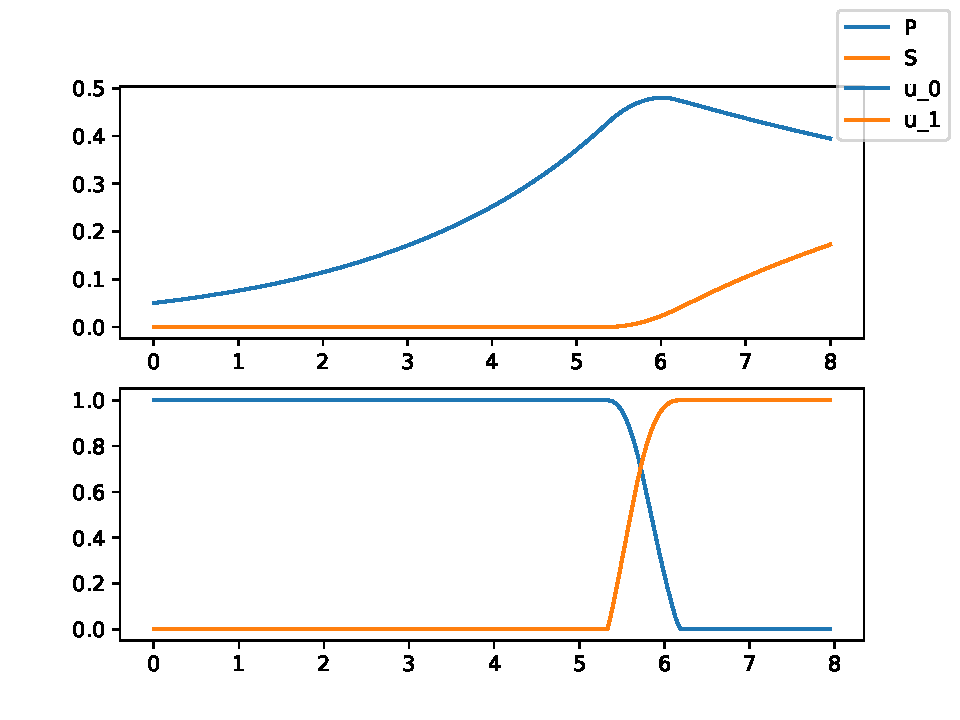
\includegraphics[width=4in]{imgs/MirmiraniOster1978_single_season.pdf}
\caption{The result of evaluating the model described in \autoref{sec:mirmirani1978-single} with parameter values $\hat{r}=0.5, \tilde{r}=0.2, \mu=0.1, \nu=0.1, T=8.0, P_0=0.05$. \label{fig:MirmiraniOster1978_single_season}}
\end{figure}

\subsection{Recovering the control}
\label{sec:control_recover}
In \autoref{sec:mirmirani1978-single} we changed the control from a multiplicative to an additive operation in order to form a convex problem. For making control plots such as those shown in \autoref{fig:MirmiraniOster1978_single_season} it is useful to map the control back to the range $[0,1]$ by taking
\begin{equation}
\begin{aligned}
\hat u_{1,t} &= \frac{u_{1,t}}{\sum_i u_{i,t}} = \frac{u_{1,t}}{\lVert u_{*,t} \rVert_1}  ~~\forall t
\end{aligned}
\end{equation}


%TODO: They, Mirmirami et al, also have competiting plants! And multi-season stuff!


\subsection{When should a plant flower?}
\label{sec:iwasa2000flower}
%TODO: Iwasa seems to have listed the wrong parameter values as evidenced by integrating g(F) from 0 to 4

\citet{Iwasa2000} considers the question of when a plant should flower, a problem first address by Cohen (1971, 1976). %TODO
Let $F(t)$ be the plant's vegetative biomass (leaves, stems and roots) and daily production (photosynthesis minus respiration) be modeled by
\begin{equation}
g(F)=\frac{aF}{1+hF}
\end{equation}
a saturating function such as this is desirable because it captures effects such as self-shading and local resource depression. Production can be allocated either to increasing vegetative biomass or reproductive biomass $R$ according to a \textit{control variable} $u(t)$. We therefore wish to solve the problem
\begin{maxi}|s|
{u(t)}{R(T)}
{}{}
\addConstraint{\dot{F}}{=(1-u)g(F)}
\addConstraint{\dot{R}}{=u g(F)}
\addConstraint{F,R}{\ge 0}
\addConstraint{F(0)}{=F_0}
\addConstraint{R(0)}{=0}
\addConstraint{u(t)}{\in[0,1]}
\end{maxi}

As usual, we will discretize and add a dimension to the control variable; however, our growth function $g(F)$ is nonlinear. We have two ways of dealing with this. Since the growth function shares a form with the Michaelis--Menten kinetics equation, we can use techniques described in \autoref{sec:mmkinetics} to convert the growth function into an SOCP constraint at the cost of some computational speed. Alternatively, we could convert the function into a piecewise-linear representation using techniques described in \autoref{sec:linearlambda}, at the cost of some accuracy. If we take the former route, our final program is:
\begin{maxi}|s|
  {u(t)}{R(T)}
  {}{}
  \addConstraint{F_{t+1}}{=F_t + \Delta t \cdot u_{t,1}}{~~\forall t}
  \addConstraint{R_{t+1}}{=R_t + \Delta t \cdot u_{t,2}}{~~\forall t}
  \addConstraint{F_t,R_t}{\ge 0}{~~\forall t}
  \addConstraint{F_{t=0}}{=F_0}
  \addConstraint{R_{t=0}}{=0}
  \addConstraint{u_{t,1} + u_{t,2}}{=g_t}{~~\forall t}
  \addConstraint{\left\lVert \begin{bmatrix} (a/h) F_t \\ (1/h) g_t \\ (a/h)(1/h) \end{bmatrix} \right\rVert_2}{\le (a/h)(1/h) + (a/h) F_t - (1/h) g_t}{~~\forall t}
\end{maxi}

While the mathematics here may seem complex, the simple Python-based modeling language we've designed for this paper makes the problem easy to express:

\inputminted[firstline=3,frame=single,linenos]{python}{src/Iwasa2000_when_flower.py}

% TODO: Philosophy of science paper. r-K selection, adding things makes them complicated. when do models get so complex you can't understand them?

% TODO: Make sure axes are labeled
% TODO: Try to make colours mean something
\begin{figure}
  \centering
  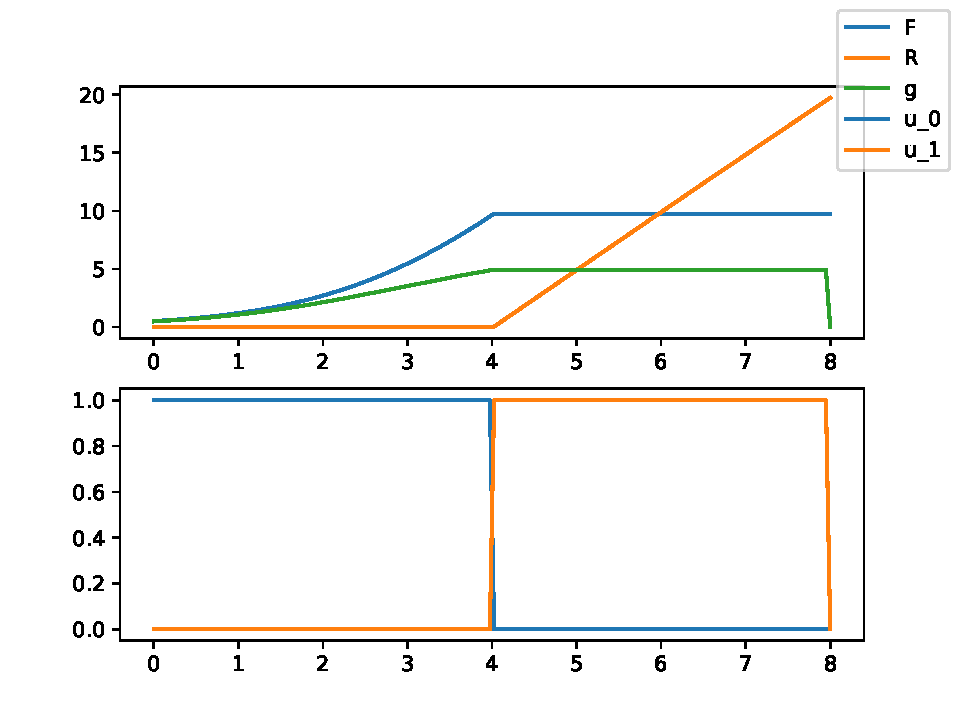
\includegraphics[width=4in]{imgs/iwasa2000_when_flower.pdf}
  \caption{The result of running the model described in \autoref{sec:iwasa2000flower} using the parameter values $a=0.1, h=1, T=8, F(0)=0.5$, following~\citep{Iwasa2000}. The control variables are normalized. \label{fig:iwasa2000flower}}
\end{figure}

The result of evaluating this model is shown in \autoref{fig:iwasa2000flower}. Analyzing the output, we see that the normalized control variables take values of either zero or one; this behaviour is called a ``bang--bang'' control. All of the plant's energy is initially used to build additional vegetative tissue (capital production); at the appropriate time all production is switched to building reproductive tissues (e.g., flowering).





\subsection{Shoot--root balance}
\label{sec:shootroot}

%TODO: Clarify
Another problem from~\citep{Iwasa1984}. Let $X_1$, $X_2$, and $R$ be the shoot, root, and accumulated reproductive biomass of a plant within a single growing season. Daily photosynthesis $g(X_1, X_2)$ will increase with the shoot biomass $X_1$ because more leaves means more photosynthesis; it will also increase with the root biomass $X_2$ because more roots means more water and nutrients. But if insufficient resources are devoted to either leaves or roots, then the plant's growth as a whole will be retarded. We can formalize the problem as:
\begin{maxi}|s|
{u(t)}{R(T)}
{}{}
\addConstraint{\dot{X_1}}{=u_1 g(X_1,X_2)}
\addConstraint{\dot{X_2}}{=u_2 g(X_1,X_2)}
\addConstraint{\dot{R}}{=u_3 g(X_1,X_2)}
\addConstraint{X_1,X_2,R}{\ge 0}
\addConstraint{u_1+u_2+u_3}{=1}
\addConstraint{X_1(0)}{=X_{1,0}}
\addConstraint{X_2(0)}{=X_{2,0}}
\addConstraint{R(0)}{=0}
\addConstraint{u_0,u_1,u_2}{\in[0,1]}
\end{maxi}
where
\begin{equation}
\label{equ:iwasa-gx1x2}
g(X_1,X_2)=\frac{1}{(a_1/LX_1^{b_1})+(a_2/WX_2^{b_2})}
\end{equation}
where $L$ is the light intensity and $W$ is the soil moisture.

If we let the shoot $S$ be $X_1$ and the root $T$ be $X_2$ then we can transform the problem as follows:
\begin{maxi}|s|
  {u(t)}{R(T)}
  {}{}
  \addConstraint{S_{t+1}}{=S_t + \Delta t \cdot u_1 }
  \addConstraint{T_{t+1}}{=T_t + \Delta t \cdot u_2 }
  \addConstraint{R_{t+1}}{=R_t + \Delta t \cdot u_3 }
  \addConstraint{S,T,R}{\ge 0}
  \addConstraint{u_1+u_2+u_3}{=g(S,T)}
  \addConstraint{S_{t=0}}{=S_0}
  \addConstraint{T_{t=0}}{=T_0}
  \addConstraint{R_{t=0}}{=0}
\end{maxi}

\begin{figure}
  \centering
  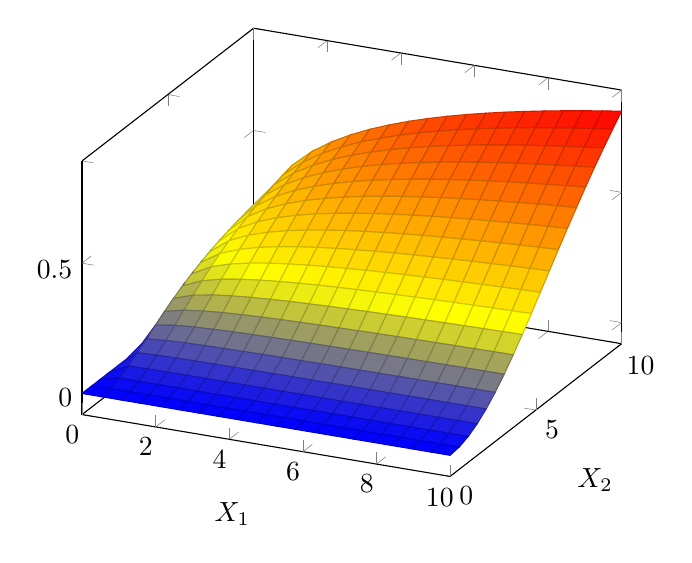
\begin{tikzpicture}
    \begin{axis}[view={25}{30},xlabel=$X_1$,ylabel=$X_2$] %Default {25}{30}
    \addplot3[surf,shader=faceted,
      samples=20,domain=0:10]
      {1/(2/1/x^0.5 + 60/1/y^2)};
    \end{axis}
  \end{tikzpicture}
  \caption{Surface plot of \autoref{equ:iwasa-gx1x2}. \label{equ:iwasa-gx1x2-splot}}
  \end{figure}


  \begin{figure}
  \centering
  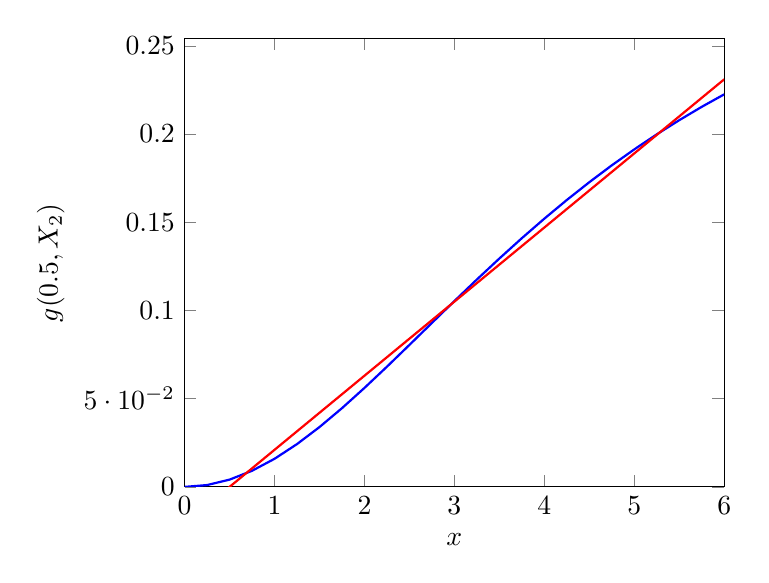
\begin{tikzpicture}
    \begin{axis}[
      xlabel=$x$,
      ylabel={$g(0.5,X_2)$},
      xmin=0,
      xmax=6,
      ymin=0,
      domain = 0:6
      % ymax=0.5,
    ]
      \addplot[thick, mark=none,blue] {1/(2/1/0.5^0.5 + 60/1/x^2)};
      \addplot[thick, mark=none,red] {0.042*(x-0.5)};
    \end{axis}
  \end{tikzpicture}
  \caption{Cross-sectional plot of \autoref{equ:iwasa-gx1x2} (blue) showing that it is non-convex (the red line passes out of the function's domain). \label{equ:iwasa-gx1x2-plot}}
\end{figure} %TODO: Prove this directly

\begin{figure}
  \centering
  \begin{tabular}{ccc}
  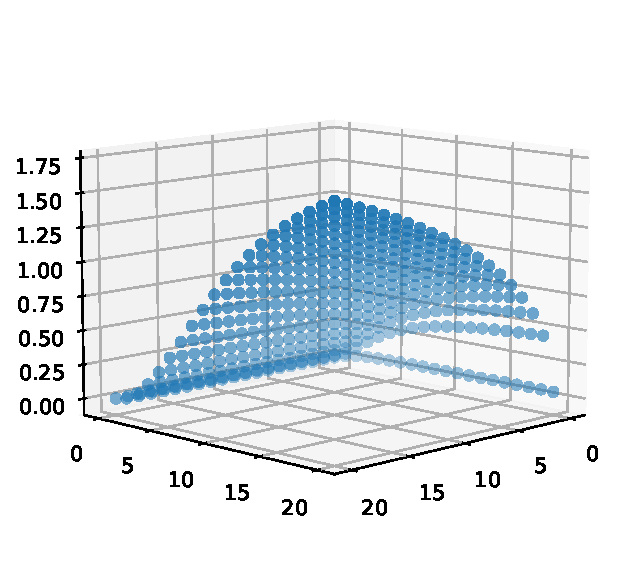
\includegraphics[width=2in]{imgs/iwasa1984_hull_samples.pdf} &
  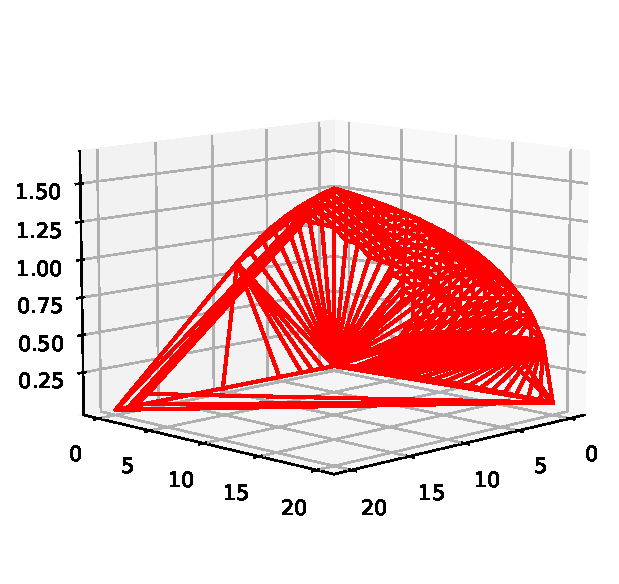
\includegraphics[width=2in]{imgs/iwasa1984_hull_full.pdf} &
  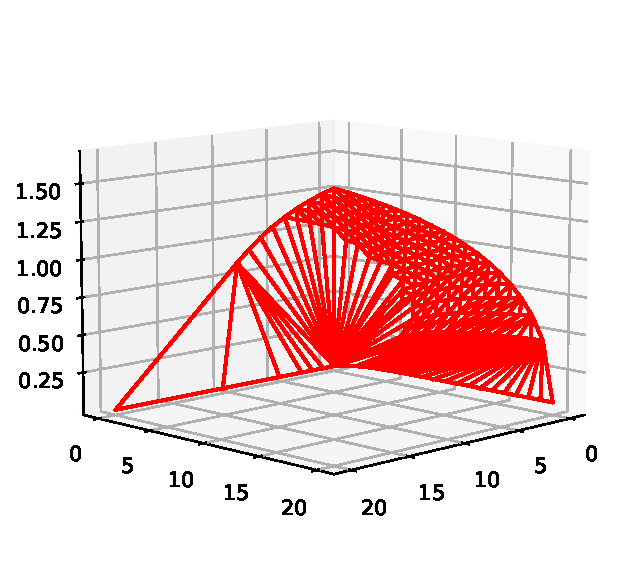
\includegraphics[width=2in]{imgs/iwasa1984_hull_upper.pdf} \\
  (a) & (b) & (c)
  \end{tabular}
  \caption{Using a convex hull to approximate a non-convex function. \textbf{(a)} points the function is sampled at. \textbf({b}) the full convex hull including all simplices; note the triangles crossing the along the bottom of the graph. \textbf({c}) the convex upper bound; note that there are no triangles crossing the bottom of the graph now. \label{fig:iwasa-hull}}
\end{figure}

%TODO: Improve discussion here. Point out that we are only justified in doing this because of the low error involved
This problem is straight-forward except for \autoref{equ:iwasa-gx1x2}, which is non-convex (\autoref{equ:iwasa-gx1x2-splot}). We can see this easily by plotting a cross-section where $X_1=0.5$ as shown in \autoref{equ:iwasa-gx1x2-plot}. To handle this situation, we sample the function $g(X_1, X_2)$ in the range $X_1=[0,X_{1,M}]$ and $X_2=[0,X_{2,M}]$ for some large values of $X_{1,M}$ and $X_{2,M}$ (\autoref{fig:iwasa-hull}a) and wrap the resulting point cloud in a convex hull (\autoref{fig:iwasa-hull}b). This returns a set of triangle simplices containing the function. Each simplex is associated with a normal vector and an offset. If we eliminate those simplices whose normal vectors have negative $z$ components this eliminates all the simplices beneath $g(\cdot)$ (\autoref{fig:iwasa-hull}c). The remaining simplices form an upper bound for $g(\cdot)$. The normals of the simplices can then be used to define a set of hyperplanes expressing this upper bound in a form amenable to mathematical programming.

\begin{figure}
\centering
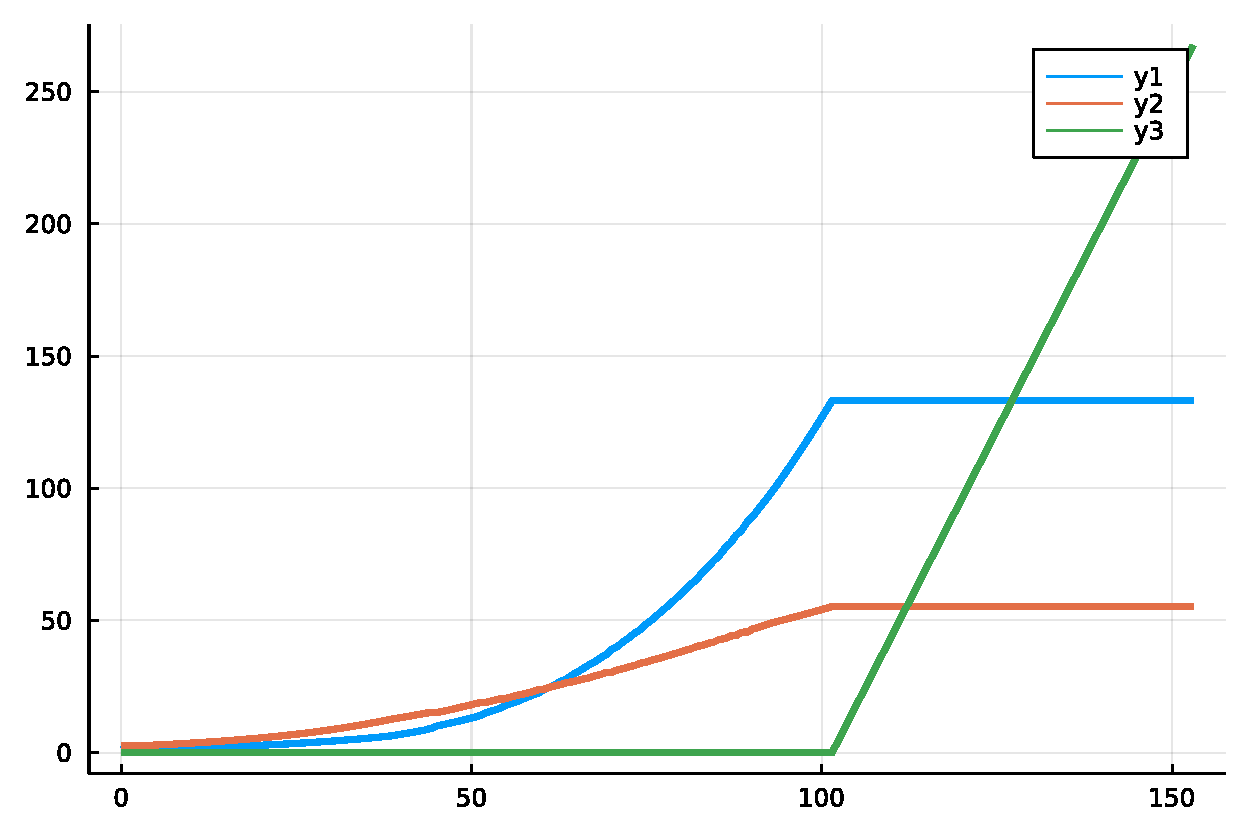
\includegraphics[width=4in]{imgs/iwasa1984_timeseries.pdf}
\caption{The optimal strategy for the model described in \autoref{sec:shootroot}.\label{fig:shootroot-result}}
\end{figure}

All this results in a large linear program which presents a formidable challenge for cvxpy's compiler. Therefore, we use Julia to gain additional performance. Following \citep{Iwasa1984}, we choose parameter values of $a_1=2, a_2=60, b_1=0.5, b_2=2,L=1,W=1, X_{1,0}=1, X_{2,0}=2.5$ to get the following program. Running it gives us the result shown in \autoref{fig:shootroot-result}.

%TODO: Show contour line and g-isolines, show costates

\inputminted[firstline=8,lastline=60,frame=single,linenos]{julia}{src/Iwasa2000_shoot_root_balance.jl}



%TODO: Add a section on separable problems.
%TODO: Add a section with more detail on piecewise approximations
%TODO: Add a section on mixed-integer linear programs
%TODO: Add a section on SOS2 constraints





%We address the problem in stages. First, we notice that the problem is not easily separable. We fix that by using neural networks to learn a separable representation of the problem using the techniques discussed in TODO. Next, we develop piecewise linear approximations of the separable representations we have learned, using the techniques discussed in TODO. Since the growth function $g$ is non-convex the SOS2 condition used in the piecewise linear approximations is not automagically satisfied, so the problem becomes a mixed-integer linear program. Nonetheless, the problem is not challenging for modern solvers.

 %TODO: See paper for back reference that might give more parameter values






\subsection{A Single Species Living Over Multiple Seasons}
\label{sec:iwasa989-multi}

\citet{Iwasa1989} present a model of a plant which can live for $n$ growing seasons ($0\le n \le\infty$), each of length $T$. The plant's vegetative tissue $F$ is the sole input to its growth function
\begin{equation}
\label{equ:iwasa1989-g}
g(F)=\frac{fF}{1+hF}
\end{equation}
where $f$ and $h$ are constants; this is the same function discussed in \autoref{sec:iwasa2000flower}. Growth is constrained such that
\begin{equation}
0\le \dot{F}\le a F_n+b
\end{equation}

The plant also has a storage tissue $S$ which encompasses bulbs, tubers, rhizomes, and similar structures which retain energy and nutrients between growing seasons, though some fraction $1-\gamma$ of this tissue is lost between growing seasons. At the end of growing season $n$ a portion $0\le R_N \le S_n$ of the storage tissue can retroactively be declared reproductive tissue.

A plausible model of growth in a single season is then
\begin{maxi}|s|
{u(t)}{S(T)}
{}{}
\addConstraint{\dot{F}}{= u(t)(aF+b)}
\addConstraint{\dot{S}}{= g(F) - u(t)(aF+b)}
\addConstraint{F(0)}{= 0}
\addConstraint{S(0)}{= S_0}
\addConstraint{F,S}{\ge 0}
\addConstraint{u(t)}{\in [0,1]}
\end{maxi}
Note that this allows biomass to move from $S$ to $F$, since $g(F)$ enters the model as an addition to $S$ and $u(t)(aF+b)$ subracts from the combined pool of $S$ and $g(F)$. Since this models a single season maximizing $S(T)$ is the same as maximizing the reproductive tissue.

To construct the multi-season model, we link single-season models together:
\begin{align}
F_n(0)     &= 0               \\
S_{n+1}(0) &= \gamma (S_{n}(T)-R_n) \\
R_n(0)     &= 0
\end{align}

The plant attempts to maximize its lifetime reproductive output:
\begin{equation}
R_\textrm{net} = \sum_{n=0}^\infty \sigma^n R_n
\end{equation}
where $0<\sigma<1$ combines the annual survival rate with any future discounting. Note that if $R_1=S_1(T)$ after optimization, then the model is indicating an annual life strategy. Similarly, if $R_2=S_2(T)$, then the plant is biennial; otherwise, the strategy is perennial.

After discretization and application of the techniques in \autoref{sec:mmkinetics} to \autoref{equ:iwasa1989-g} we get the following mathematical program:
\begin{maxi}|s|
{u(t)}{\sum_{n=0}^Y \sigma^n R_n}
{}{}
\addConstraint{F_{n,t+1}}{= F_{n,t} + \Delta t \cdot u_{n,t}}
\addConstraint{S_{n,t+1}}{= S_{n,t} + \Delta t \left( g_{n,t} - u_{n,t} \right)}
\addConstraint{\left\lVert \begin{bmatrix} (f/h) F_t \\ (1/h) g_{n,t} \\ (f/h)(1/h) \end{bmatrix} \right\rVert_2}{\le (f/h)(1/h) + (f/h) F_t - (1/h) g_{n,t}}{~~\forall t}
\addConstraint{F_{n,0}}{= 0}
\addConstraint{S_{0,0}}{= S_0}
\addConstraint{S_{n+1,0}}{= \gamma (S_{n,T}-R_n)}
\addConstraint{F,S,R}{\ge 0}
\addConstraint{u_{n,t}}{\ge0}
\addConstraint{u_{n,t}}{\le aF_{n,t}+b}
\end{maxi}
Though we would like $Y=\infty$, our mathematical modeling framework cannot handle this. However, this is not a severe restriction. Consider a relatively large value for $\sigma$ such as 0.85. After 10 years the discount rate is 0.19 and, after 20 years, it has become 0.038. That is, the plant's reproductive value 20 years out is worth only 3.8\% of the value of the plant's reproductive output during its first year of life. $\sigma$ is necessarily greater than zero, otherwise the plant has no incentive to grow; $\sigma$ is also necessarily less than one because the future is risky and no plant can guarantee its survival.

\begin{figure}
\centering
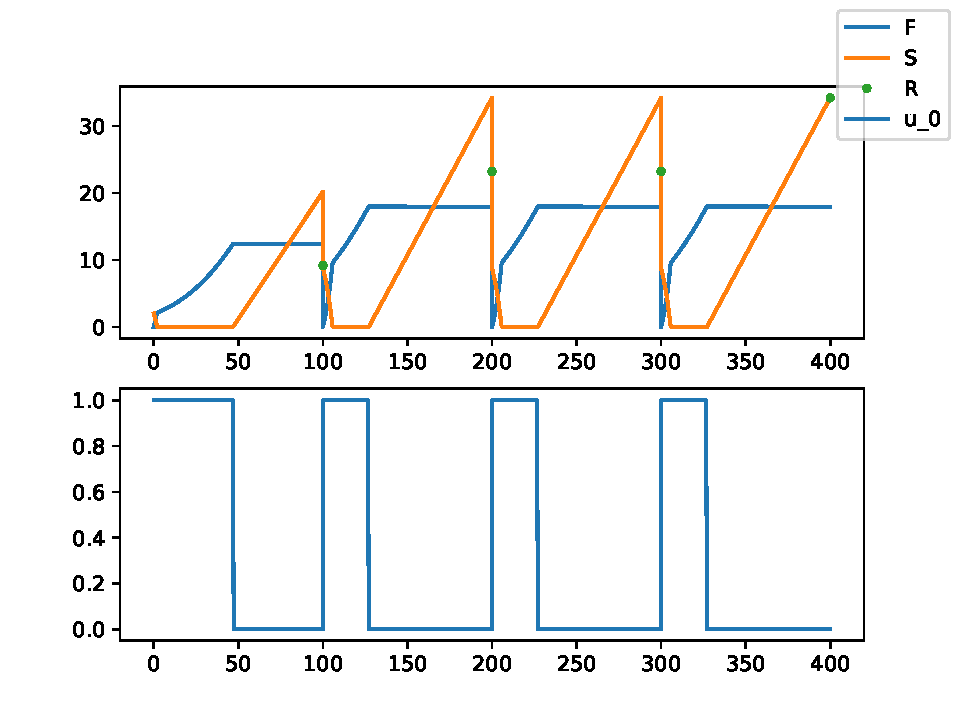
\includegraphics[width=4in]{imgs/Iwasa1989_multi_season.pdf}
\caption{The result of evaluating the model described in \autoref{sec:iwasa989-multi} with parameter values $a=0.2, b=1, f=0.05, h=0.05, T=100, S_0=2, \gamma=0.8$ over four years. \label{fig:iwasa1989-multi}}
\end{figure}

In this paper's modeling language the problem instantiates as:

\inputminted[firstline=3,frame=single,linenos]{python}{src/Iwasa1989_multi_season.py}

Solving this gives the result shown in \autoref{fig:iwasa1989-multi}. The growth pattern of the plant shows that during its first year of life it preserves about half of its storage to jump-start growth in subsequent years. During the next few years, the plant enters a recurring pattern which is only broken during the last year when the finite time horizon cause it to put all of its energy into reproduction. The plant's control variable is again bang-bang.

%TODO: Talk about and show three-phase and two-phase growth



\subsection{Environmental Effects}

\citet{mironchenko_optimal_2014} present a flexible growth model coupled with more realistic depictions of seasonality and time-varying effects. This flexibility gives them the ability to determine under what conditions a variety of life histories are optimal. The model is
\begin{equation}
\begin{aligned}
\dot x_1 &= v_1(t)g(x_3) - \mu(t) x_1                  \\
\dot x_2 &= \left(v(t)-v_1(t)\right)g(x_3)             \\
\dot x_3 &= \zeta(t)f(x_1) - v(t)g(x_3) -\omega(t)x_3
\end{aligned}
\end{equation}
where $x_1$ is vegetative tissue, $x_2$ is reproductive tissue, $x_3$ is storage tissue, $v\in[0,1]$ and $v_1\in[0,v]$ are control variables allocating storage tissue at a maximal rate of $g(x_3)$, $f(x_1)$ is the rate of photosynthesis in optimal environment conditions, $\zeta(t)$ models the dependence of the photosynthetic rate on the environment ($\zeta(t)=0$ implies no photosynthesis is possible), $\mu(t)$ is the loss rate of vegetative tissues, and $\omega(t)$ is the loss rate of storage tissues.

The optimal rate of photosynthesis, $f(x)$, always has the form
\begin{equation}
f(x) = \frac{ax}{bx+k}
\end{equation}
while the achievable fraction of photosynthesis, $\zeta(t)$, remains the same throughout the systems \citeauthor{mironchenko_optimal_2014} test:
\begin{equation}
\zeta(t) = 0.2 + 0.8 \left\lvert \sin \left(\frac{\pi}{12}t\right)\right\rvert
\end{equation}
its periodic form might represent, e.g., seasonal temperature variation. $\mu$ and $\omega$ often have periodic forms as well.

To convert this model to our form, we note that the control variables $v$ and $v_1$ apportion up to $g(x_3)$ energy between $x_1$ and $x_2$. Therefore, we can replace them with two control variables $u_1,u_2\ge 0$ constrained such that $u_1+u_2\le g(x_3)$. Doing this and discretizing per usual gives us the system:
\begin{maxi}|s|
  {u(t)}{x_{2,T}}
  {}{}
  \addConstraint{x_{1,t+1}}{= x_{1,t} + \Delta t \cdot \left(u_{1,t} - \mu(t) x_1 \right)}
  \addConstraint{x_{2,t+1}}{= x_{2,t} + \Delta t \cdot u_{2,t}}
  \addConstraint{x_{3,t+1}}{= x_{3,t} + \Delta t \cdot \left(\zeta(t) f(x_{1,t}) - u_{1,t} - u_{2,t} - \omega(t) x_{3,t}\right)}
  \addConstraint{x_{1,0}}{= 0.05 m}
  \addConstraint{x_{2,0}}{= 0     }
  \addConstraint{x_{3,0}}{= 0.95 m}
  \addConstraint{u_{1,t}+u_{2,t}}{\le g(x_3)}
\end{maxi}
where $m$ is the initial seed mass. The introduction of the time-varying functions $\zeta,\omega,\mu$ don't make our modeling job more difficult. Since we've discretized over time, we can just evaluate these functions at each time point and insert the result as a constant into our model.

\subsubsection{Inducing Multiple Reproduction Periods}
\label{sec:annual-multi}
What is the effect of periodic vegetative tissue loss on an annual, as might be caused by herbivores grazing repeatedly over the same area as it regrows? To answer this, \citeauthor{mironchenko_optimal_2014} instantiate the above model for two environments

\begin{center}
\begin{tabular}{lcc}
\textbf{Variable} & \textbf{Stable Environment}                 & \textbf{Unstable Environment}     \\
$\omega(t)=$      & $0.05$                                      & $t / (1 + 0.5 t)$                 \\
$\mu(t)=$         & $0.8 \lvert \cos(\frac{\pi}{12}t) \rvert$   & $1.8 \lvert \cos(\pi t) \rvert$   \\
$g(x_3)=$         & $5x_3$                                      & $16x_3$                           \\
$f(x_1)=$         & $1.5x/(1+0.03x_1)$                          & $4x/(1+0.03x_1)$                  \\
Outcome           & Single reproductive period                  & Multiple reproductive periods
\end{tabular}
\end{center}

Note that while the stable environment has a $\mu(t)$ that's periodic over the course of a year, as would be the case for seasonal vegetative loses, the unstable environment has a $\mu(t)$ that varies monthly, perhaps as levels of herbivory fluctuate. To survive this stability the plant in the unstable environment needs a higher maximum storage conversion rate $g(x_3)$ and greater optimal photosynthetic efficiency $f(x_1)$. The unstable plant's $\omega(t)$ was chosen by \citeauthor{mironchenko_optimal_2014} as a saturating function to help emphasize the control variables and costates.

In this paper's modeling language the above becomes:

\inputminted[firstline=5,frame=single,linenos]{python}{src/Mironchenko2014_figure2.py}

Running the above program gives us the result shown in \autoref{fig:mironchenko-fig2}. Note that the low levels of vegetative tissue lost in the stable environment result in continuous reproductive output, even though the loss levels are fluctuating. Even though the unstable environment is more favourable for the plant, having greater photosynthesis and faster storage conversion, strong fluctuations in vegetative tissue loss result in pulsed reproductive output.

\begin{figure}
  \centering
  \begin{tabular}{cc}
    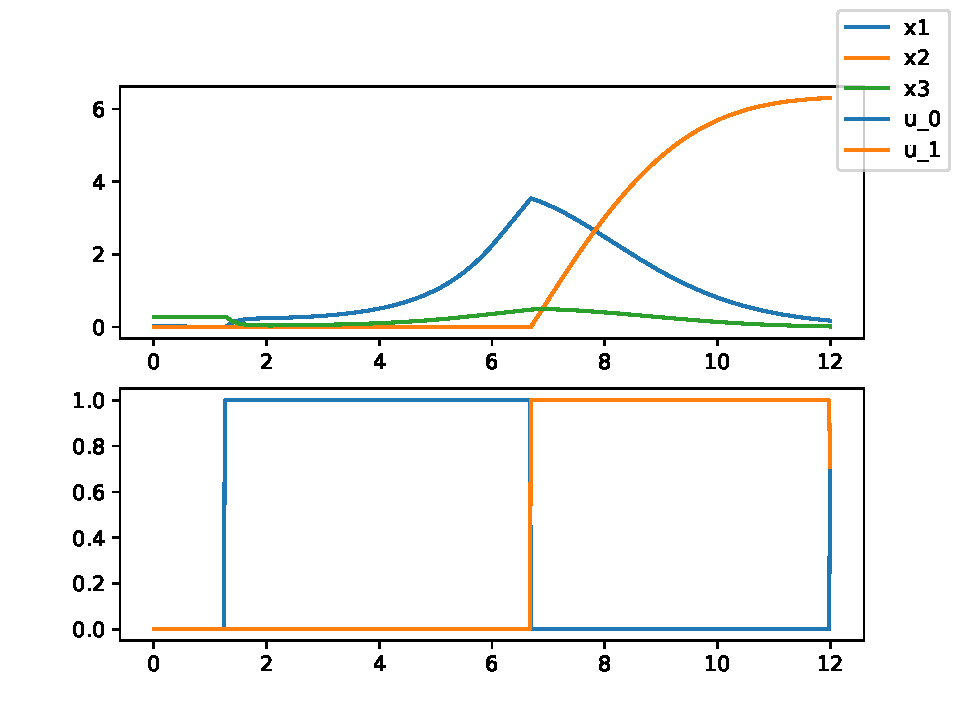
\includegraphics[width=3in]{imgs/Mironchenko_figure2a.pdf} &
    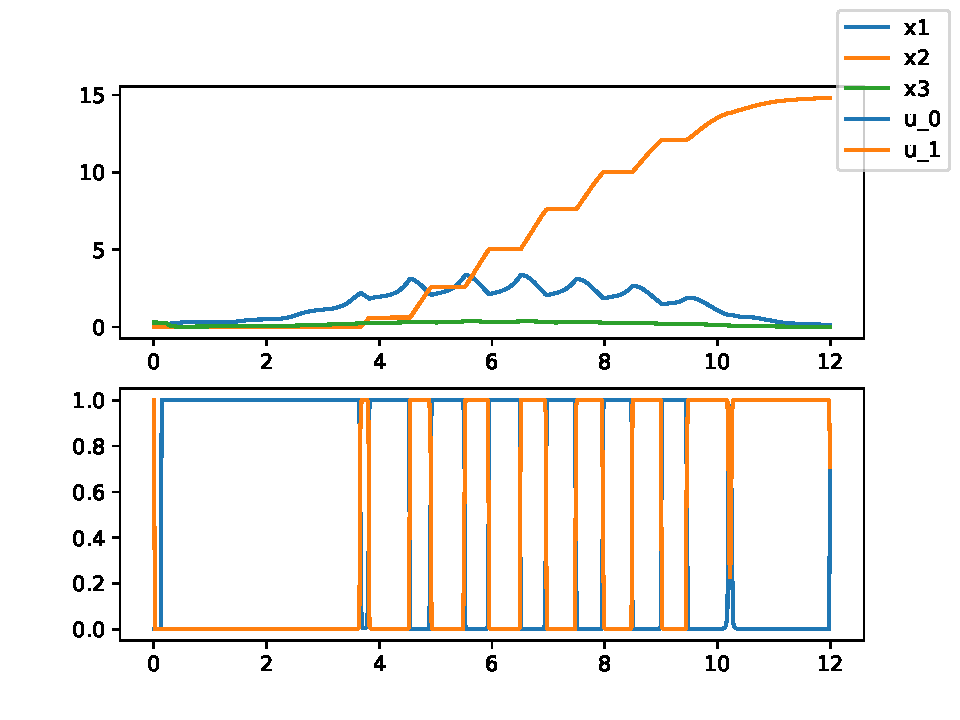
\includegraphics[width=3in]{imgs/Mironchenko_figure2b.pdf} \\
    (a) & (b)
  \end{tabular}
  \caption{The result of evaluating the model described in \autoref{sec:annual-multi}. \textbf{(a)} shows an annual plant growing in a stable environment whereas \textbf{(b)} shows an annual plant growing in an unstable environment. The results match Figure 2 of \citep{mironchenko_optimal_2014}.\label{fig:mironchenko-fig2}}
\end{figure}

% If we very the severity of tissue loss during the winter, we can force a plant to switch from an annual to a perennial strategy:
% \begin{center}
% \begin{tabular}{lcc}
% \textbf{Variable} & \textbf{Low Winter Losses}                            & \textbf{High Winter Losses}       \\
% $\omega(t)=$      & $1.6\lvert\cos\left(\frac{\pi}{12}(t-6)\right)\rvert$ & $t / (1 + 0.5 t)$                 \\
% $\mu(t)=$         & $2.4\lvert \cos(\frac{\pi}{12}t) \rvert$              & $1.8 * \lvert \cos(\pi t) \rvert$ \\
% $g(x_3)=$         & $5x_3$                                                & $16x_3$                           \\
% $f(x_1)=$         & $2.5/(1+0.01x_1)$                                     & $4/(1+0.03x_1)$                   \\
% Outcome           & Annual
% \end{tabular}
% \end{center}
% TODO: Seed stage



% TODO MONOCARP In a TODO environment specified by
% \begin{center}
% \begin{tabular}{lcc}
% \textbf{Variable} & \textbf{Stable Env}                         & \textbf{Unstable Env}             \\
% $\omega(t)=$      & 0.1                                         & $t / (1 + 0.5 t)$                 \\
% $\mu(t)=$         & $0.4 * \lvert \cos(\frac{\pi}{12}t) \rvert$ & $1.8 * \lvert \cos(\pi t) \rvert$ \\
% $g(x_3)=$         & $2.5x_3$                                    & $16x_3$                           \\
% $f(x_1)=$         & $0.5/(1+0.01x_1)$                           & $4/(1+0.03x_1)$
% \end{tabular}
% \end{center}

\subsubsection{Perennial Strategies}
\label{sec:miron-per-strat}

%TODO: Seed mass
We can generate a variety of perennial strategies by varying the environment:
\begin{center}
\begin{tabular}{lcccc}
\textbf{Variable} & \textbf{Constantly Harsh}                & \textbf{Constant Mortality}     & \textbf{Pleasant}                 & \textbf{Very Pleasant}          \\
Seed Mass         & 0.3                                      & Same                            & Same                              & Same                            \\
Seed Fractions    & $<5\%, 0\%, 95\%>$                       & Same                            & Same                              & Same                            \\
$\omega(t)=$      & $0.15$                                   & 0, see below                    & 1                                 & 0.1                             \\
$\mu(t)=$         & $0.4\lvert \cos(\frac{\pi}{12}t) \rvert$ & $0.4 \lvert \cos(\pi t) \rvert$ & $0.1 \lvert \cos(\pi t) \rvert$   & $0.4 \lvert \cos(\pi t) \rvert$ \\
$g(x_3)=$         & $2.5x_3$                                 & Same                            & Same                              & Same                            \\
$f(x_1)=$         & $0.5/(1+0.1x_1)$                         & Same                            & Same                              & $0.5/(1+0.01x_1)$               \\
Outcome           & Storage                                  & No storage                      & Storage                           & Monocarpy
\end{tabular}
\end{center}
We can instantiate these environments in this paper's modeling language through minor modifications to the program shown in \autoref{sec:annual-multi}.

As shown in \autoref{fig:mironchenko-fig5ae}, the ``Constantly Harsh" environment causes the plant to lose significant vegetative tissue over winters. It makes up for this by moving energy into storage. The ``Constant Mortality" produces a similar result via a different means. For this, we set $\omega(t)=0$, but model the plant has having a 3\% chance of dying at any given moment. This implies that the probability $L(t)$ of surviving to an age $t$ is given by $L(t)=e^{-0.03t}$. The plant's goal is then to maximize its expected lifetime fitness, which is given by
\begin{equation}
\int_0^T L(t) \dot x_2(t) dt
\end{equation}
incorporating this into our modeling language is straight-forward
\inputminted[firstline=37,lastline=38,frame=single]{python}{src/Mironchenko2014_figure5e.py}

Contrast this with the the ``Pleasant'' and ``Very Pleasant'' environments, as shown in \autoref{fig:mironchenko-fig4and5c}. The decreased over-winter tissue loss ($\mu$) in the pleasant environment means that even though storage losses ($\omega$) are smaller, the plant's best strategy is to accept some tissue losses rather than waste energy on using storage. In the ``Very Pleasant" environment, the plant is again subject to higher over-winter tissue loss ($\mu$), but storage costs are very low. The biggest difference, though is that the plant has minimal self-shading. This is modeled by choosing a maximum photosynthetic rate ($f$) with a denominator ($1+0.01x_1$) that is small for most values of $x_1$ the plant will encounter.



\begin{figure}
  \centering
  \begin{tabular}{ccc}
    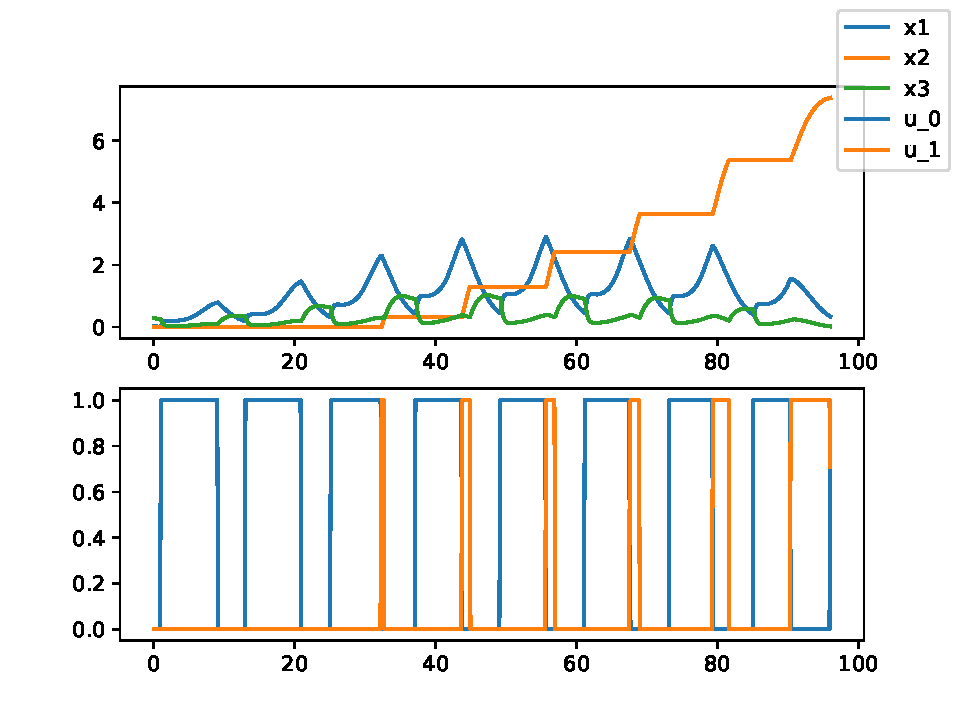
\includegraphics[width=3in]{imgs/MironchenkoFigure5a.pdf} &
    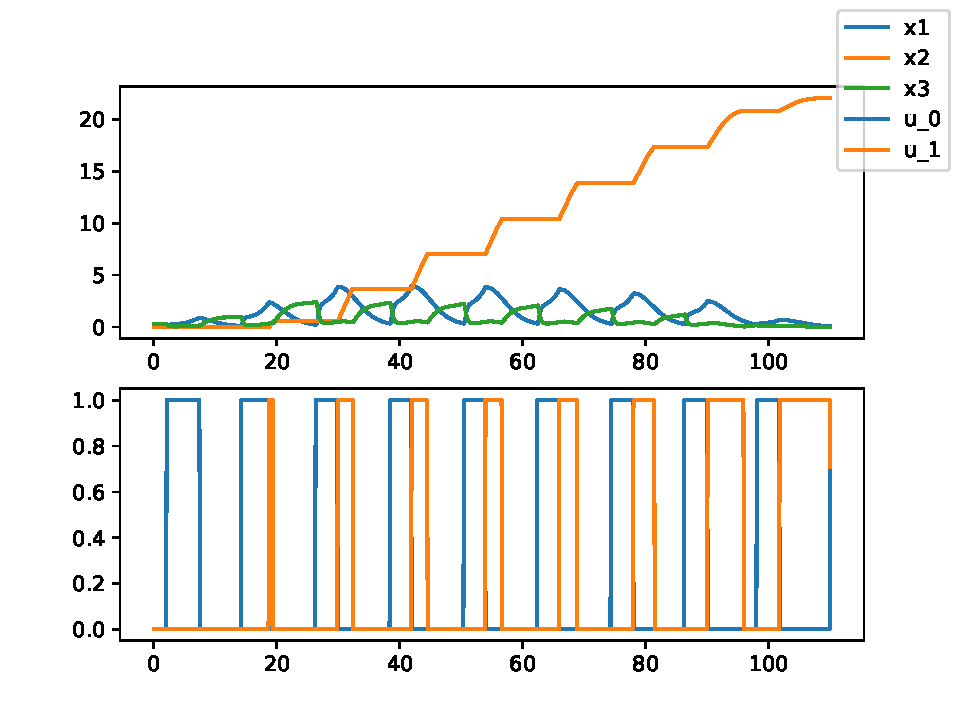
\includegraphics[width=3in]{imgs/MironchenkoFigure5e.pdf} \\
    (a) & (b)
  \end{tabular}
  \caption{The result of evaluating the ``Constantly Harsh'' \textbf{(a)} and ``Constant Mortality'' \textbf{(b)} environments described in \autoref{sec:miron-per-strat}. Both environments have similar optimal strategies. The results match Figure 5a of \citep{mironchenko_optimal_2014} exactly and Figure 5e nearly (see the note on reproducibility TODO).\label{fig:mironchenko-fig5ae}}
\end{figure}

\begin{figure}
  \centering
  \begin{tabular}{ccc}
    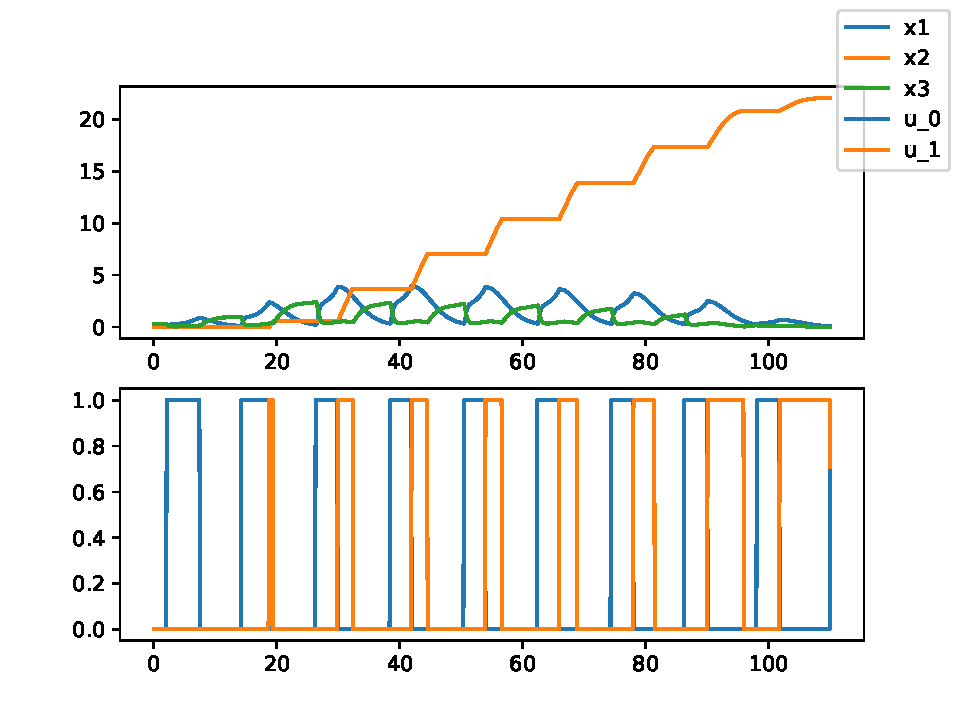
\includegraphics[width=3in]{imgs/MironchenkoFigure5e.pdf} &
    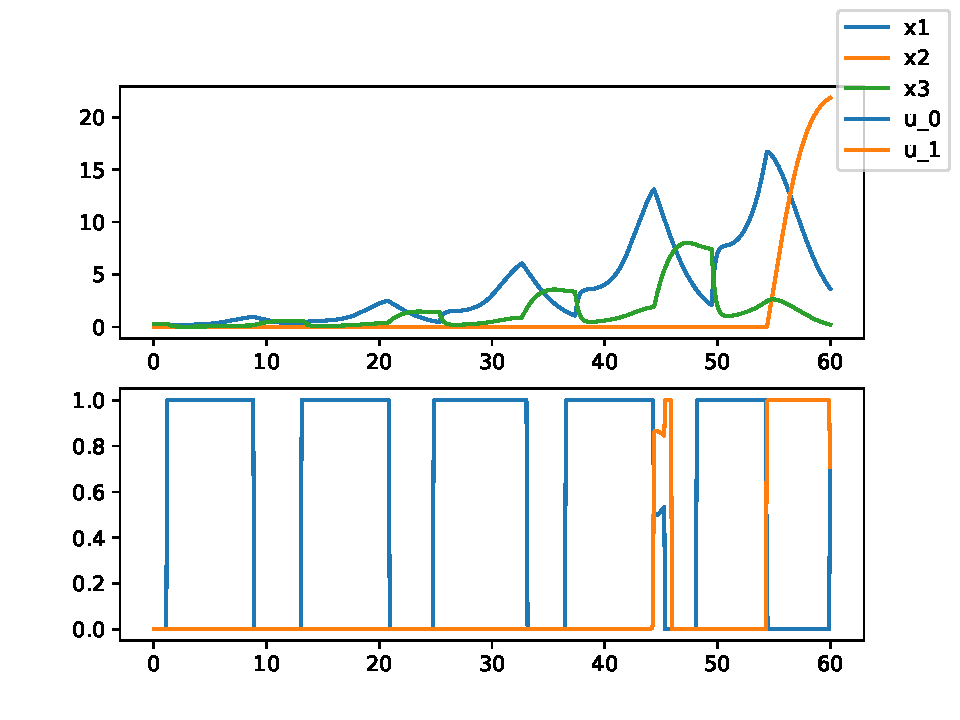
\includegraphics[width=3in]{imgs/Mironchenko_figure4.pdf} \\
    (a) & (b)
  \end{tabular}
  \caption{The result of evaluating the ``Pleasant" \textbf{(a)} and ``Very Pleasant" \textbf{(b)} environments in \autoref{sec:miron-per-strat}. The plant requires uses almost no storage in the pleasant environment while in the very pleasant environment it chooses monocarpy as a strategy. The results match Figure 4 and Figure 5c of \citep{mironchenko_optimal_2014}.\label{fig:mironchenko-fig4and5c}}
\end{figure}


\begin{comment}
\subsection{Two Species Competing In A Single Season}

%TODO: Better explain the motivation for the following equations

\citet{mirmirani_competition_1978} explore two species competing in a single season. Let the biomass of the vegetative parts of the plants be $P_1$ and $P_2$, the biomass of the reproductive tissues $S_1$ and $S_2$, $E_1$ and $E_2$ the strength of the competitive interactions, and $r_1$ and $r_2$ are assimilation constants. The growth of the plants can then be modeled as (\citep[Eq.\ 4--1 -- 4--4]{mirmirani_competition_1978})
\begin{align}
\dot{P_1} &= (r_1-E_2 P_2) u_1 P_1 \\
\dot{P_2} &= (r_2-E_1 P_1) u_2 P_2 \\
P_1(0)      &=P_{1,0}>0 \\
P_2(0)      &=P_{2,0}>0 \\
r_1-E_2 P_2 &\ge 0 \\
r_2-E_1 P_1 &\ge 0 \\
\dot{S_1} &= (r_1-E_2 P_2) (1 - u_1) P_1 \\
\dot{S_2} &= (r_2-E_1 P_1) (1 - u_2) P_2 \\
S_1(0)&=0 \\
S_2(0)&=0 \\
u_1, u_2 & \in [0,1]
\end{align}
If we set $E=E_1=E_2$, $r=r_1=r_2$, and $P_0=P_{1,0}=P_{2,0}$ and then renormalize $P_1\rightarrow EP_1$ and $P_2\rightarrow EP_2$, then the equations simplify to (\citep[Eq.\ 4--4 -- 4--8]{mirmirani_competition_1978})
\begin{align}
  \dot{P_1} &= (r-P_2) u_1 P_1 \\
  \dot{P_2} &= (r-P_1) u_2 P_2 \\
  P_1(0)      &=P_{1,0}>0 \\
  P_2(0)      &=P_{2,0}>0 \\
  r-P_2 &\ge 0 \\
  r-P_1 &\ge 0 \\
  \dot{S_1} &= (r-P_2) (1 - u_1) P_1 \\
  \dot{S_2} &= (r-P_1) (1 - u_2) P_2 \\
  S_1(0)&=0 \\
  S_2(0)&=0 \\
  u_1, u_2 & \in [0,1]
\end{align}
Per usual, we add a dimension to the control variable:
\begin{align}
  \dot{P_1} &= (r-P_2) u_{1,1} \\
  \dot{P_2} &= (r-P_1) u_{2,1} \\
  P_1(0)      &=P_{1,0}>0 \\
  P_2(0)      &=P_{2,0}>0 \\
  r-P_2 &\ge 0 \\
  r-P_1 &\ge 0 \\
  \dot{S_1} &= (r-P_2) u_{1,2} \\
  \dot{S_2} &= (r-P_1) u_{2,2} \\
  S_1(0)&=0 \\
  S_2(0)&=0 \\
  u_{1,1} + u_{1,2} &= P_1 \\
  u_{2,1} + u_{2,2} &= P_2
\end{align}

\end{comment}


%TODO: Parameter sweeps

%TODO: Discuss and demonstrate dual/shadow values for variables and constraints (can cvxpy show these?)

%TODO: Disciplined parameter programming (solve same problem many times quickly)

%TODO: Failure modes (infinity when maximizing means unbounded)


\section{Inverse Problems}
\label{sec:inverse_problem_mirmir}

Given a noisy sampling of a timeseries can we recover the underlying system? To explore this, let's start with a system where we know the system. We'll use the simple single-season system described in \autoref{sec:mirmirani1978-single}.

To make a noisy problem, we solve the single-season system, add normally distributed noise to one of the result variables, and then sample a few data points to get a vector of scalar values $P_\textrm{noise,sampled}$. Previously, our objective was to maximize the amount of seeds at the end of the season $\max S(T)$. Our new objective tries to match the system, as described by the vector of variables $P$, to the data. This gives us the objective
\begin{equation}
\min_u \lVert P_\textrm{noise,sampled} - P \rVert_2
\end{equation}
we can implement this as follows:
\inputminted[firstline=12,lastline=26,frame=single,linenos]{python}{src/MirmiraniOster1978_inverse_problem.py}
running this gives us the result shown in \autoref{fig:mirmir-fit}a.



\begin{figure}
  \centering
  \begin{tabular}{ccc}
    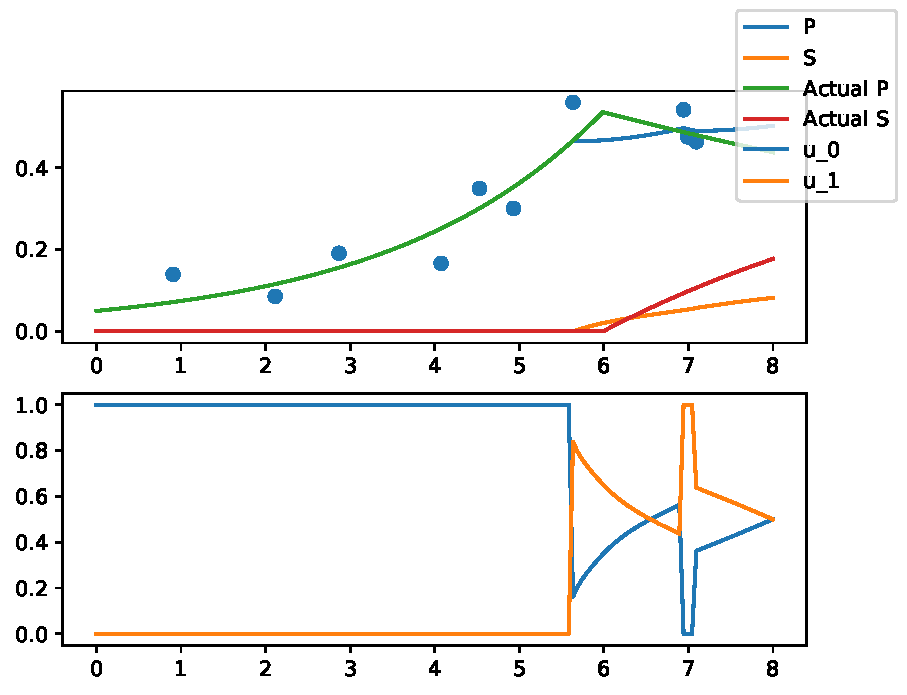
\includegraphics[width=3in]{imgs/Mirmirani_inverse_bad_fit.pdf} &
    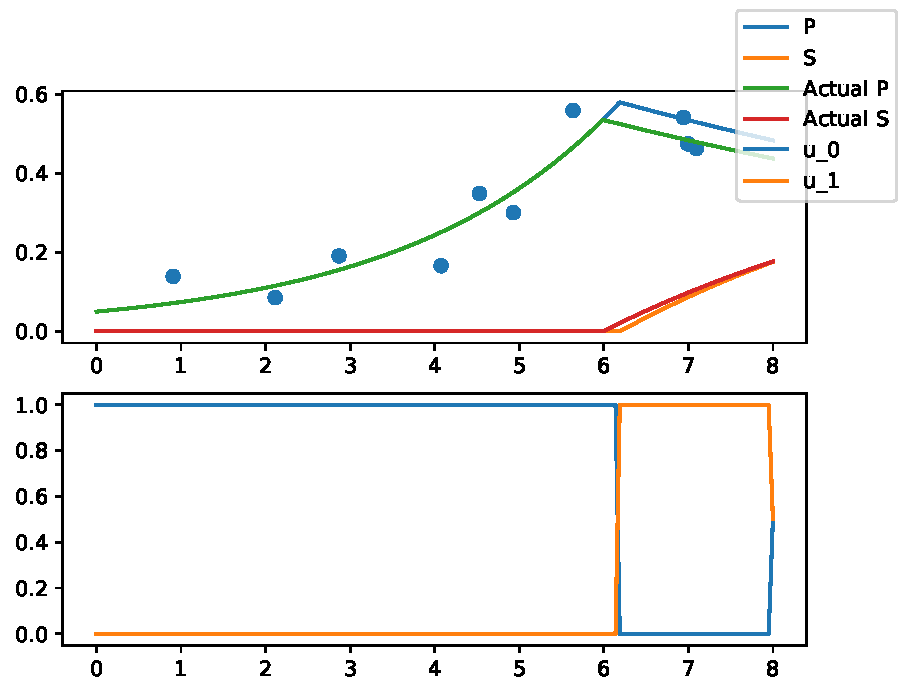
\includegraphics[width=3in]{imgs/Mirmirani_inverse_good_fit.pdf} \\
    (a) & (b)
  \end{tabular}
  \caption{The result of solving the inverse problem described in \autoref{sec:inverse_problem_mirmir}. \textbf{(a)} shows the result when the inverse problem is solved without any constraints on the control variable. \textbf{(b)} shows the result when the inverse problem is solved with the control variable constrained to switch only two times. \label{fig:mirmir-fit}}
\end{figure}

The optimal solution of the system for this new least-squares objective is overfit: the system is able to follow the noise and sparsity of the data. However, we have a strong prior that the system has a bang-bang control. \citet{Burger2020} provides us a method for recovering the optimal bang-bang control strategy. First, we solve the problem with no constraints on the control. This gives us continuous-valued outputs for the controls. Second, we solve a \textit{combinatorial integral approximation} (CIA) problem. The inputs for this problem are the discretized timepoints which we used to approximation the differential equations and the values of the controls, mapped to the range $[0,1]$, resulting from the relaxed problem. The CIA problem allows us to specify constraints such as the number of times a control should switch from on to off. Since we have a prior expectation from \autoref{sec:mirmirani1978-single} that this should happen only once per growing season, we add that as a constraint. The result of solving the CIA problem is a set of bang-bang control values. Third, and finally, we solve our least-squares problem again, but this time with the constraint that the control must follow the bang-bang values we obtained from the CIA.

These steps require some subtly since a key part step in the conversion from differential to convex forms so far has been manipulating the control from a multiplicative to an additive factor. \autoref{sec:control_recover} explains how to recover $[0,1]$ controls to get the input to the CIA. We then note that the control constraint for \autoref{sec:mirmirani1978-single} is
\begin{equation}
u_{1,t}+u_{2,t}=P_t~~\forall t
\end{equation}
If we call the bang-bang controls returned from the CIA $\hat u$, then the following additional constraints ensure that our system follows strategy prescribed by the CIA
\begin{equation}
\begin{aligned}
u_{1,t}&=\hat u_{1,t} P_t~~\forall t \\
u_{2,t}&=\hat u_{2,t} P_t~~\forall t
\end{aligned}
\end{equation}

We can implement all this as follows:

\inputminted[firstline=40,lastline=61,frame=single,linenos]{python}{src/MirmiraniOster1978_inverse_problem.py}

As shown in \autoref{fig:mirmir-fit}, using the CIA least-squares approach allows us to recover almost exactly the original system.





\section{Techniques}
\label{sec:techniques}

%\subsection{The Forward-Euler Method}
%\label{sec:euler}

%TODO


\subsection{Bilinear Constraints}

%TODO: From http://minlp.cheme.cmu.edu/2014/papers/castro.pdf
% Pedro M. Castro of Universidade de Lisboa seems to have put it together
\begin{figure}
\centering
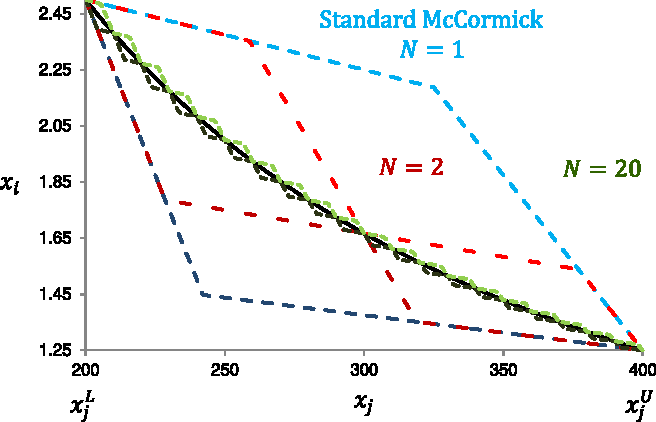
\includegraphics[width=4in]{imgs/piecewise_mccormick.pdf}

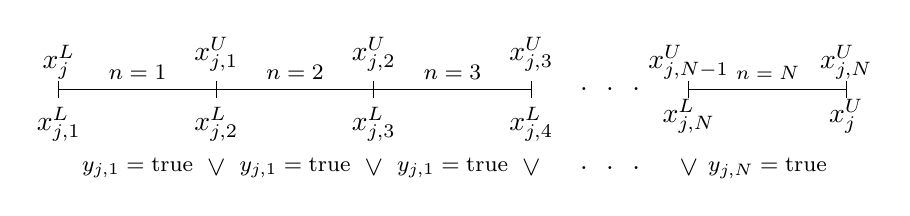
\begin{tikzpicture}
  \draw[-] (2*1,0) -- (2*4,0) ; % edit here for the axis
  \foreach \x in  {1,2,3,4} % edit here for the vertical lines
  \draw[shift={(2*\x,0)},color=black] (0pt,3pt) -- (0pt,-3pt);

  \foreach \x in  {1,2,3} % edit here for the vertical lines
  \node[above] at ({2*\x+2*0.5},0) {\footnotesize $n=\x$};

  \foreach \x in  {1,2,3} % edit here for the vertical lines
  \node at ({2*\x+2*0.5},-1) {\footnotesize $y_{j,1}=\textrm{true}$};
  \node at ({2*5+2*0.5},-1) {\footnotesize $y_{j,N}=\textrm{true}$};
  \node at (2*2,-1) {$\vee$};
  \node at (2*3,-1) {$\vee$};
  \node at (2*4,-1) {$\vee$};
  \node at (2*4+2*0.5,-1) {.~~.~~.};
  \node at (2*5,-1) {$\vee$};

  \draw[-] (2*5,0) -- (2*6,0) ; % edit here for the axis
  \foreach \x in {5,6} % edit here for the vertical lines
  \draw[shift={(2*\x,0)},color=black] (0pt,3pt) -- (0pt,-3pt);

  \foreach \x in {1,2,3,4} % edit here for the numbers
  \draw[shift={(2*\x,0)},color=black] (0pt,0pt) -- (0pt,-3pt) node[below]
  {$x_{j,\x}^L$};
  \foreach \x in {1,2,3} % edit here for the numbers
  \draw[shift={({2*(\x+1)},0)},color=black] (0pt,0pt) -- (0pt,3pt) node[above]
  {$x_{j,\x}^U$};

  \node at (2*4+2*0.5,0) {.~~.~~.};

  \node[above] at ({2*5+2*0.5},0) {\scriptsize $n=N$};

  \node[above] at (2*5,0) {$x_{j,N-1}^U$};
  \node[below] at (2*5,0) {$x_{j,N}^L$};
  \node[above] at (2*6,0) {$x_{j,N}^U$};

  \node[above] at (2*1,0) {$x_j^L$};
  \node[below] at (2*6,0) {$x_j^U$};

\end{tikzpicture} %TODO: Discuss the number line here. Optimization will pick a single segment. Domain divide into N uniform partitions
\caption{Piecewise McCormick Envelopes\label{fig:piecewise_mccormick}}
\end{figure}

A bilinear constraint is one in which we require that $w=xy$ where both $x$ and $y$ are variables. A common way to handle such a constraint is by enclosing it in concave and convex bounds known as McCormick envelopes, as shown in \autoref{fig:piecewise_mccormick}. Unfortunately, these bounds are often loose. This can be handled either by iteratively refining the bounds or by using mixed-integer programming to generate a series of small envelopes. This can be expressed via a \textit{generalized disjunctive program (GDP)}: %TODO: Cite Balas (1979); Raman & Grossman (1994)
\begin{gather}
x_{jn}^L = x_j^L + (x_j^U-x_j^L) \frac{n-1}{N} \\
x_{jn}^U = x_j^L + (x_j^U-x_j^L) \frac{n}{N} \\
x_i^L \le x_i \le x_i^U \\
\bigvee_n\begin{bmatrix}
y_{jn} \\
w_{ij} \ge x_i\cdot x_{jn}^L + x_i^L \cdot x_j - x_i^L \cdot x_{jn}^L \\
w_{ij} \ge x_i\cdot x_{jn}^U + x_i^U \cdot x_j - x_i^U \cdot x_{jn}^U \\
w_{ij} \le x_i\cdot x_{jn}^L + x_i^U \cdot x_j - x_i^U \cdot x_{jn}^L \\
w_{ij} \le x_i\cdot x_{jn}^U + x_i^L \cdot x_j - x_i^L \cdot x_{jn}^U \\
x_{jn}^L \le x_j \le x_{jn}^U
\end{bmatrix} \\
y_{jn}\in\{\textrm{True},\textrm{False}\} \\
\Omega(y) = \textrm{True}
\end{gather}
While some optimization DSLs can handle GDPs natively, we can re-express this is a MILP so that we solve it using a wide variety of solvers and DSLs~\citep{Grossman2012}.
\begin{align}
x_{jn}^L &= x_j^L + (x_j^U-x_j^L) \frac{n-1}{N} \\
x_{jn}^U &= x_j^L + (x_j^U-x_j^L) \frac{n}{N} \\
x_i^L &\le x_i \le x_i^U \\
-w_{ij} + x_i\cdot x_{jn}^L + x_i^L \cdot x_j - x_i^L \cdot x_{jn}^L &\le M(1-y_{jn}) \\
-w_{ij} + x_i\cdot x_{jn}^U + x_i^U \cdot x_j - x_i^U \cdot x_{jn}^U &\le M(1-y_{jn}) \\
w_{ij} - x_i\cdot x_{jn}^L - x_i^U \cdot x_j + x_i^U \cdot x_{jn}^L &\le M(1-y_{jn})  \\
w_{ij} - x_i\cdot x_{jn}^U - x_i^L \cdot x_j + x_i^L \cdot x_{jn}^U &\le M(1-y_{jn})  \\
x_{jn}^L - x_j &\le M(1-y_{jn}) \\
x_j - x_{jn}^U &\le M(1-y_{jn}) \\
\sum_j y_{jn} &= 1 \\
y_{jn}&\in\{0,1\}
\end{align}
%TODO: Discuss convex hull formulation shown in https://link.springer.com/content/pdf/10.1007/s10898-012-0022-1.pdf
%TODO: Above takes waaaay too long with CBC for even 100 timesteps


%TODO: Probably don't need this because we really want bilinear
\subsection{Hyperbolic constraints}

\subsubsection{As SOCPs}

For a vector $\vec{w}$ a constraint of the form
\begin{equation}
\vec{w}^T\vec{w}=\lVert\vec{w}\rVert^2_2\le xy,~~~x\ge0,~~~y\ge0
\end{equation}
can be transformed into the SOCP constraint
\begin{equation}
\label{equ:hyperbolic-to-socp}
\left\lVert \begin{bmatrix} 2\vec{w} \\ x - y \end{bmatrix} \right\rVert_2 \le x+y
\end{equation}
Note that the optimal value of a scalar $w$ produced this way is the squart root of $xy$.

% \subsection{Converting square roots to SOCPs}

% A constraint of the form
% \begin{equation}
% \sqrt{x}\ge t
% \end{equation}
% can be transformed into the SOCP constraints
% \begin{equation}
% \left\lVert \begin{bmatrix} 1-x \\ 2t \end{bmatrix} \right\rVert_2 \le 1+x
% \end{equation}



\subsection{Michaelis--Menten Kinetics}
\label{sec:mmkinetics}

%TODO: DIscuss cvxpy atom solution

The Michaelis--Menten relates the rate $y$ of an enzymatic reaction to the concentration $x$ of a substrate, as follows
\begin{equation}
\label{equ:mm}
Y = \frac{\beta_1 X}{\beta_2 + X}
\end{equation}
where $\beta_1$ and $\beta_2$ are positive parameters.

\autoref{equ:mm} most often appears in our context as a saturating limit to growth, e.g., $\textrm{growth}\le\frac{\beta_1 X}{\beta_2 + X}$. Since optimizing reproductive fitness often means maximizing growth, we anticipate that the inequality will be binding. \autoref{equ:mm} is therefore equivalent to the hyperbolic constraint
\begin{align}
\label{equ:mm-hyper}
\hat{X}^2+\hat{Y}^2 &\le (\hat{X}-\hat{Y})(2\beta_1\beta_2+\hat{X}-\hat{Y}) \\
   0    &\le \hat{X}-\hat{Y}
\end{align}
were $\hat{X}=\beta_1 X$ and $\hat{Y}=\beta_2Y$; this can be proven by simplifying \autoref{equ:mm-hyper}. Converting this to the standard SOC form using \autoref{equ:hyperbolic-to-socp} gives
\begin{equation}
\left\lVert \begin{bmatrix} \hat{X} \\ \hat{Y} \\ \beta_1\beta_2 \end{bmatrix} \right\rVert_2 \le \beta_1\beta_2 + \hat{X} - \hat{Y}
\end{equation}
and substituting in $\hat{X}$ and $\hat{Y}$ gives
\begin{equation}
\left\lVert \begin{bmatrix} \beta_1 X \\ \beta_2 Y \\ \beta_1\beta_2 \end{bmatrix} \right\rVert_2 \le \beta_1\beta_2 + \beta_1 X - \beta_2 Y
\end{equation}

Note that if our M-M kinetics equation is instead
\begin{equation}
  Y = \frac{\beta_1 X}{\beta_2 + \beta_3 X}
\end{equation}
we can convert to the canonical form by taking
\begin{equation}
  Y = \frac{(\beta_1/\beta_3) X}{(\beta_2/\beta_3) + X}
\end{equation}

An application of this technique to gradostat design is discussed in~\citep{Taylor2021}.



\subsection{SOS2 Constraints}
\label{sec:sos2}

An SOS2 constraint is defined by specifying a set of variables $\{t_1,t_2,\ldots,t_n\}$ and is equivalent to the following three constraints:
\begin{itemize}
\item $t_1,t_2,\ldots,t_n\ge0$
\item $t_1+t_2+\ldots+t_n=1$
\item At most two adjacent variables, $t_i$ and potentially $t_{i+1}$ can be non-zero
\end{itemize}
SOS2 constraints are useful for modeling piecewise-linear functions, as described in \autoref{sec:linearlambda}. If a solver doesn't have SOS2 constraints but has binary variables, these can be used to construct an equivalent, though less efficient, formulation.



\subsection{Linearizing Functions}
\label{sec:linearlambda}

%TODO: The importance of separable functions in a mathematical programming model lies in the fact that they can be approximated to by piecewise linear functions. It is then possible to use separable programming to obtain a global optimum to a convex problem or possibly only a local optimum for a non-convex problem.

One way to handle a non-linear function $f(x)$ is to approximate it as a piecewise-linear function of $n$ line segments using a standard $\lambda$-form transformation~\citep{Williams2013}. For $f(x)$ in the range $[a,b]$ and a step size $s=(b-a)/n$, we add the following constraints to the model: %TODO: See Williams, p. 149
\begin{align}
x &= \sum_{i=0}^{n-1}  (a+is) \lambda_{i} \\
y &= \sum_{i=0}^{n-1} f(a+is) \lambda_{i} \\
1 &= \sum_{i=0}^{n-1}         \lambda_{i} \\
&\textrm{at most two adjacent $\lambda_{i}$ can be nonzero} \label{equ:adjlambda}
\end{align}
now, $y$ is a linear approximation of $f(x)$ and can be used in its place anywhere in the model. The constraint given by \autoref{equ:adjlambda} is nonlinear. However, if $f(x)$ has diminishing returns and we are maximizing our objective then this constraint is guaranteed to be true and need not be explicitly included in the model~\citep{Williams2013}. (Once the model has been solved, the values of $\lambda$ can be checked as a verification measure.) For cases where the above doesn't hold, most solvers include \textit{SOS2} constraints as a way to enforce \autoref{equ:adjlambda} (see \autoref{sec:sos2}).








%NOTE: First found this proof here: https://arxiv.org/pdf/2102.01975.pdf


\begin{comment}
import cvxpy as cp

S=cp.Variable()
T=cp.Variable()

# We use cp.SOC(t, x) to create the SOC constraint ||x||_2 <= t.

a = cp.SOC(2+S-T, cp.vstack([S,T,1]))
#a = (x*x+y*y<=(x-y)*(2+x-y))
b = (0<=x-y)
\end{comment}

\begin{comment}
The Michaelis--Menten relates the rate $y$ of an enzymatic reaction to the concentration $x$ of a substrate, as follows
\begin{equation}
y = \frac{\beta_1 X}{\beta_2 + X}
\end{equation}
where $\beta_1$ and $\beta_2$ are positive parameters.
%SEE: https://arxiv.org/pdf/2102.01975.pdf !!!!! TODO TODO TODO, Equation 12a

There are several ways to linearize this equation.

The Eadie--Hofstee linearization
\begin{equation} %TODO: Check per https://en.wikipedia.org/wiki/Eadie%E2%80%93Hofstee_diagram
y=-\beta_2\frac{y}{x}+\beta_1
\end{equation}
The Hanes--Wolf linearization:
\begin{equation} %TODO: Check per https://en.wikipedia.org/wiki/Hanes%E2%80%93Woolf_plot
\frac{x}{y}=\frac{1}{\beta_1}x+\frac{\beta_2}{\beta_1}
\end{equation}
The Lineweaver--Burk linearization: %TODO: Substituting for 1/y and 1/x looks promising maybe
\begin{equation} %TODO: Check per https://en.wikipedia.org/wiki/Lineweaver%E2%80%93Burk_plot
\frac{1}{y}=\frac{\beta_2}{\beta_1}\frac{1}{x}+\frac{1}{\beta_1}
\end{equation}
The ``inverse" Eadie--Hofstee linearization:
\begin{equation}
x=\beta_1\frac{x}{y}-\beta_2
\end{equation}
\end{comment}


%TODO: See http://www.seas.ucla.edu/~vandenbe/publications/socp.pdf for chance and robust constraints
%TODO: http://citeseerx.ist.psu.edu/viewdoc/download?doi=10.1.1.94.9988&rep=rep1&type=pdf for chance and robust constraints



\begin{comment}
The predictions are made by extending multi-season resource allocation models based on optimal control theory to account for a range of competitive pressures. Such models assume (1)~that plants must allocate energy and nutrients to different organs, (2)~that these organs have separate functions such that allocations represent hard trade-offs, %Find a better phrase than "hard trade-offs". Use "mutually exclusive", maybe?
and (3)~that the timing and quantity of allocations evolve to maximize an individual's lifetime reproductive output weighted by a yearly survival probability. %Find a more generalized phrase than "risk discounting". Think about "individual plant's"
\end{comment}


{\footnotesize
\bibliographystyle{abbrvnat}
\bibliography{refs,theory}
}


\end{document}


%TODO: Make sure greek letters appear in minted/code outputs
%TODO: Talk about costates!
%TODO: Talk about collocation or RK45 or other more accurate discretizations of the differential equations

%Acknowledgements: Gerpheides for hosting me in Dec 2021. Eleanor for hosting me while I started the mathematical programming work.
